\part{Des histoires à l'observation}
\chapter{Des trajectoires aux histoires}\label{t3-des-trajectoires-aux-histoires}

Le Tome II s'est achevé sur une question de composition.

À chaque histoire $\mathcal H$ était associée une fonction de réponse
\[
\mathcal R_{\mathcal H}(u)
=
\left(
T^\ast_{\mathcal H}(u),
g_{\mathrm{app},\mathcal H}(u),
\mathcal A_{\infty,\mathcal H}(u)
\right),
\]
et la possibilité d'une dépendance à l'ordre était formulée par
\[
\mathcal R_{\mathcal H_1\cdot\mathcal H_2}
\stackrel{?}{=}
\mathcal R_{\mathcal H_2\cdot\mathcal H_1}.
\]

Cette écriture indiquait déjà le problème, mais elle ne suffisait pas encore à le poser complètement.

En effet, une différence entre les deux membres peut avoir plusieurs origines. Elle peut résulter d'une simple pondération de récence, d'une non-commutativité effective des expériences, ou d'une modification plus profonde de la manière dont le système répond désormais aux interventions futures. Ces mécanismes ne peuvent être distingués à partir de la seule comparaison de deux trajectoires.

Il faut d'abord préciser ce que l'on appelle une histoire, ce qui en survit dans l'état présent, et selon quelles lectures deux histoires peuvent être considérées comme fonctionnellement distinctes.

Le Tome III prend donc pour objet non plus seulement l'évolution d'un système, mais la relation entre les transformations qu'il a traversées et l'espace de ses réponses futures.

La question directrice devient alors :
\begin{quote}
\itshape À quelles conditions deux réalisations d’un même système initial, soumises à des histoires différentes, demeurent-elles séparables par leurs réponses futures ?
\end{quote}
La séparation ne porte donc pas directement sur les passés eux-mêmes, mais sur les transformations qu’ils ont laissées dans les réalisations du système et sur les différences de réponse que des interventions ultérieures permettent encore de révéler.

Cette progression conduira successivement à :

\begin{itemize}
\tightlist
\item
  définir les histoires et leurs lectures ;
\item
  isoler leur contenu survivant ;
\item
  déterminer quand un état lent suffit à en résumer les effets ;
\item
  décrire les frontières où les réponses changent ;
\item
  distinguer les propriétés du comportement de celles de sa présentation ;
\item
  construire enfin une géométrie de la séparabilité entre histoires.
\end{itemize}

Le point de départ reste celui posé à la fin du Tome II : une trajectoire individuelle ne se caractérise pas seulement par les attracteurs déjà atteints, mais par la manière dont les interactions passées ont modifié l'accessibilité des attracteurs futurs.

Le premier pas consiste maintenant à donner un sens formel au mot
\emph{histoire}.

\section{Pourquoi la trajectoire ne suffit pas}
\label{t3-pourquoi-la-trajectoire-ne-suffit-pas}

Une trajectoire décrit l'évolution effective d'une réalisation du système. Elle ordonne les états traversés, les événements rencontrés et les transformations produites au cours du temps.

Cette description ne suffit toutefois pas à caractériser ce que le système est devenu.

Deux réalisations peuvent atteindre des états instantanés proches, voire identiques au regard des variables observées, tout en ne répondant plus de la même manière aux interventions ultérieures. Inversement, deux trajectoires très différentes peuvent conduire à des réalisations que plus aucune sonde admissible ne permet de distinguer.

La différence entre les trajectoires passées n'est donc ni une condition suffisante ni une condition nécessaire de la séparabilité future.

Le problème du Tome III ne consiste pas à comparer directement des chemins dans l'espace d'état. Il consiste à déterminer ce que ces chemins ont laissé dans les réalisations qui les ont suivis.

Soit une réalisation initiale $X_0$, soumise à une histoire $\mathcal H$. À l'issue de cette histoire, on obtient une réalisation transformée que l'on peut noter provisoirement
\[
X_{\mathcal H}.
\]

Cette notation ne suppose pas que toute l'histoire soit encodée dans un état instantané, ni qu'elle puisse être reconstruite à partir de celui-ci. Elle indique seulement que les réponses futures du système peuvent dépendre de l'histoire qu'il a traversée.

Soumise à une intervention ultérieure $u$, la réalisation
$X_{\mathcal H}$ produit une réponse
\[
\mathcal R_{\mathcal H}(u).
\]

Deux histoires $\mathcal H_1$ et $\mathcal H_2$, appliquées à deux réalisations comparables du même système initial, demeurent fonctionnellement séparables s'il existe au moins une intervention admissible $u$ telle que
\[
\mathcal R_{\mathcal H_1}(u)
\neq
\mathcal R_{\mathcal H_2}(u).
\]

La comparaison porte ainsi sur un diagramme de la forme
\[
X_0
\;\xrightarrow{\;\mathcal H_j\;}\;
X_{\mathcal H_j}
\;\xrightarrow{\;u\;}\;
\mathcal R_{\mathcal H_j}(u),
\qquad j\in\{1,2\}.
\]

L'histoire intervient donc à deux niveaux distincts.

D'une part, elle décrit une succession effective de transformations. D'autre part, elle désigne ce qui, dans cette succession, demeure encore capable de modifier les réponses futures.

Ces deux niveaux ne doivent pas être confondus. Une partie du passé peut avoir eu lieu sans demeurer fonctionnellement active. À l'inverse, une transformation brève peut laisser une modification persistante de l'accessibilité des régimes futurs.

Il faut dès lors distinguer trois objets :

\begin{itemize}
\tightlist
\item
  la trajectoire effectivement parcourue ;
\item
  l'histoire en tant que composition de transformations ;
\item
  le contenu de cette histoire qui survit dans les réponses futures.
\end{itemize}

La première étape consiste à préciser le deuxième de ces objets. Le contenu survivant ne pourra être défini qu'une fois établi ce qui compte comme une histoire, comment plusieurs épisodes s'y composent, et selon quelles lectures cette histoire est interrogée.

\section{Histoires, épisodes et composition}
\label{t3-histoires-episodes-composition}

Une histoire n'est pas introduite comme une trajectoire continue supplémentaire. Elle décrit l'ordre dans lequel une réalisation du système traverse une suite d'épisodes susceptibles de la transformer.

Soit $\mathcal E$ l'ensemble des épisodes admissibles. À chaque épisode $e\in\mathcal E$ est associée une application de transition
\[
\Phi_e:\mathfrak X\longrightarrow\mathfrak X,
\]
où $\mathfrak X$ désigne l'espace dans lequel est représentée la réalisation du système.

Une histoire finie est un mot
\[
\mathcal H=e_1e_2\cdots e_n.
\]
Elle se lit de gauche à droite dans l'ordre chronologique : le système vit d'abord $e_1$, puis $e_2$, et ainsi de suite jusqu'à $e_n$.

La transformation induite par cette histoire est
\[
\Phi_{\mathcal H}
=
\Phi_{e_n}\circ\cdots\circ\Phi_{e_1}.
\]
L'histoire vide est notée $\varepsilon$ et vérifie
\[
\Phi_{\varepsilon}
=
\operatorname{Id}_{\mathfrak X}.
\]

Cette distinction entre l'ordre d'écriture de l'histoire et l'ordre de composition des applications sera conservée dans tout le Tome III.

Si $\mathcal H_1$ et $\mathcal H_2$ sont deux histoires, leur concaténation
\[
\mathcal H_1\cdot\mathcal H_2
\]
désigne l'histoire dans laquelle le système vit d'abord $\mathcal H_1$, puis $\mathcal H_2$. Par conséquent,
\begin{equation}
\label{eq:t3-composition-histoires}
\boxed{
\Phi_{\mathcal H_1\cdot\mathcal H_2}
=
\Phi_{\mathcal H_2}\circ\Phi_{\mathcal H_1}.
}
\end{equation}

L'histoire et la transition qu'elle induit ne doivent cependant pas être identifiées.

Deux histoires différentes peuvent produire la même transformation :
\[
\mathcal H_1\neq\mathcal H_2,
\qquad
\Phi_{\mathcal H_1}
=
\Phi_{\mathcal H_2}.
\]
Dans ce cas, leur différence chronologique ne laisse aucune différence dans la réalisation finale, du moins à l'échelle décrite par $\mathfrak X$.

Réciproquement, deux transitions distinctes peuvent ne pas être distinguées par les réponses que l'on choisit d'observer :
\[
\Phi_{\mathcal H_1}
\neq
\Phi_{\mathcal H_2},
\]
sans qu'il existe nécessairement, parmi les sondes admissibles, une intervention $u$ telle que
\[
\mathcal R_{\mathcal H_1}(u)
\neq
\mathcal R_{\mathcal H_2}(u).
\]

Trois niveaux de comparaison apparaissent ainsi :

\begin{itemize}
\tightlist
\item
  la différence entre les mots historiques ;
\item
  la différence entre les transitions qu'ils induisent ;
\item
  la différence entre les réponses futures que les sondes permettent
  effectivement de révéler.
\end{itemize}

Ces niveaux ne coïncident pas en général.

La question de l'ordre formulée à la fin du Tome II doit donc être précisée. Au niveau des histoires, elle oppose
\[
\mathcal H_1\cdot\mathcal H_2
\qquad\text{et}\qquad
\mathcal H_2\cdot\mathcal H_1.
\]
Au niveau des transitions, elle devient
\[
\Phi_{\mathcal H_2}\circ\Phi_{\mathcal H_1}
\stackrel{?}{=}
\Phi_{\mathcal H_1}\circ\Phi_{\mathcal H_2}.
\]
Au niveau des réponses futures, elle s'écrit
\[
\mathcal R_{\mathcal H_1\cdot\mathcal H_2}(u)
\stackrel{?}{=}
\mathcal R_{\mathcal H_2\cdot\mathcal H_1}(u)
\]
pour les interventions admissibles $u$.

Une différence observée au dernier niveau établit que l'ordre demeure fonctionnellement détectable. Elle ne suffit toutefois pas à identifier le mécanisme qui la produit.

Dans le modèle actuel, l'épisode vécu en dernier peut peser davantage sur l'état lent simplement parce que son effet a subi moins d'atténuation. L'échange de deux épisodes modifie alors la réponse sans qu'il soit encore nécessaire d'invoquer une restructuration durable de l'organisation interne.

Il faut donc distinguer deux affirmations :

\begin{enumerate}
\item
  l'ordre des épisodes modifie la réponse future ;
\item
  l'histoire a modifié de manière persistante la façon dont le système transforme les interventions futures.
\end{enumerate}

La première porte sur une différence observable. La seconde porte sur la nature de ce qui survit à l'histoire. Elle exige davantage qu'une simple comparaison entre deux états terminaux ou entre deux valeurs instantanées de la fonction de réponse.

Le problème n'est donc plus seulement de savoir si
\[
\mathcal H_1\cdot\mathcal H_2
\quad\text{et}\quad
\mathcal H_2\cdot\mathcal H_1
\]
produisent des résultats différents. Il est de déterminer quelle part de cette différence demeure active, sous quelles interventions elle peut être révélée, et si elle peut être expliquée par le seul écoulement du temps.

La notion d'histoire étant désormais posée, il reste à préciser comment elle est interrogée. Une différence passée ne devient fonctionnellement pertinente qu'à travers les lectures capables d'en révéler les effets.

\section{Sondes, lectures et séparabilité relative}
\label{t3-sondes-lectures-separabilite}

Une différence entre deux réalisations ne devient fonctionnellement pertinente que si une intervention permet de la révéler et si une lecture permet d'en comparer les effets.

Il faut donc distinguer ce que l'on fait vivre au système de ce que l'on observe de son exécution.

\subsection{Toute sonde est une histoire}

Soit
\[
\mathfrak M=\mathcal E^\ast
\]
le monoïde des histoires finies introduit précédemment. Un protocole d'observation déclare une classe
\[
\mathfrak B\subseteq\mathfrak M
\]
d'histoires admissibles.

Une sonde n'est donc pas nécessairement une intervention instantanée. Elle peut comprendre une exposition, une attente, une regraine, une relaxation ou une composition de plusieurs de ces épisodes. Elle est elle-même une histoire.

\subsection{Ce qu'une sonde permet de lire}

Lorsqu'une réalisation $X$ est soumise à une histoire de sonde $\mathcal H$, elle produit une exécution
\[
\operatorname{Exec}_{\mathcal H}(X).
\]

Cette exécution rassemble tout ce qui s'est produit pendant la sonde : la trajectoire continue, les événements éventuels, les états avant et après chaque saut, ainsi que l'état terminal.

Une expérience ne retient cependant pas nécessairement toute cette information.

Elle peut, par exemple, observer seulement :

\begin{itemize}
\tightlist
\item
  l'attracteur finalement atteint ;
\item
  le nombre de Kairos produits ;
\item
  leur calendrier ;
\item
  ou une portion particulière de la trajectoire.
\end{itemize}

On note $\rho$ le choix de ce qui est ainsi retenu. Dans la suite, $\rho$ désignera donc une \emph{lecture}, ou de manière équivalente une résolution d'observation.

Le symbole $\rho$ ne décrit pas une variable interne du système. Il appartient au protocole utilisé pour l'interroger.

Pour une lecture fixée, la réponse observée est notée
\[
\mathcal R_X^\rho(\mathcal H).
\]

Le passage de l'exécution à la réponse peut être représenté par
\[
\operatorname{Exec}_{\mathcal H}(X)
\;\xrightarrow{\;\rho\;}\;
\mathcal R_X^\rho(\mathcal H).
\]

Une lecture terminale ne conserve que ce qui peut être déterminé à partir de l'état atteint à la fin de la sonde. Elle peut notamment indiquer le bassin terminal ou l'attracteur rejoint.

Une lecture de chemin conserve au contraire une information produite pendant l'exécution : le nombre d'événements, leur ordre, leur calendrier ou certaines caractéristiques de la trajectoire.

Deux réalisations peuvent ainsi atteindre le même attracteur tout en l'atteignant par des chemins différents. Elles seront indiscernables pour une lecture terminale qui ne conserve que l'attracteur, mais pourront être séparées par une lecture de chemin plus fine.

Inversement, deux exécutions mathématiquement différentes peuvent conduire à la même réponse lorsque la lecture choisie ne conserve pas ce qui les distingue.

La réponse dépend donc de trois éléments :
\[
\text{la réalisation interrogée},
\qquad
\text{l'histoire de sonde},
\qquad
\text{la lecture retenue}.
\]

L'écriture employée à la fin du Tome II peut maintenant être précisée.

Lorsque l'état initial $X_0$, la lecture $\rho$ et une famille de sondes paramétrées par $u$ sont laissés implicites, l'expression
\[
\mathcal R_{\mathcal H_0}(u)
\]
désigne la réponse obtenue après qu'une réalisation initiale a vécu l'histoire $\mathcal H_0$, puis a été soumise à la sonde associée à $u$.

En développant les éléments restés implicites, cette réponse s'écrit
\[
\mathcal R_{\Phi_{\mathcal H_0}(X_0)}^\rho
\bigl(\mathcal H_u\bigr).
\]
\subsection{Une équivalence déclarée}
\label{t3-equivalence-declaree}

Une fois fixées les histoires de sonde admissibles et la lecture retenue, la comparaison de deux réalisations devient précise.

Soient deux réalisations
\[
X,Y\in\mathfrak X.
\]

Elles sont dites \emph{équivalentes en réponse} relativement à la classe de sondes \(\mathfrak B\) et à la lecture \(\rho\) lorsque toute histoire admissible produit la même réponse à partir de $X$ et de $Y$ :
\begin{equation}
\label{eq:t3-equivalence-observationnelle}
\boxed{
X\sim_{\mathfrak B,\rho}Y
\quad\Longleftrightarrow\quad
\forall\mathcal H\in\mathfrak B,
\qquad
\mathcal R_X^\rho(\mathcal H)
=
\mathcal R_Y^\rho(\mathcal H).
}
\end{equation}

Cette définition ne compare donc pas directement les états internes de $X$ et de $Y$. Elle compare ce qu'ils donnent à voir lorsqu'ils sont soumis aux mêmes histoires de sonde et lus de la même manière.

À l'inverse, les deux réalisations sont séparables dans le protocole déclaré s'il existe au moins une histoire
\[
\mathcal H\in\mathfrak B
\]
telle que
\[
\mathcal R_X^\rho(\mathcal H)
\neq
\mathcal R_Y^\rho(\mathcal H).
\]

Une telle histoire sera dite \emph{séparatrice} pour $X$ et $Y$ à la lecture $\rho$.

La séparabilité possède ainsi un témoin explicite :
\[
X\not\sim_{\mathfrak B,\rho}Y
\quad\Longleftrightarrow\quad
\exists\mathcal H\in\mathfrak B
\ \text{telle que}\
\mathcal R_X^\rho(\mathcal H)
\neq
\mathcal R_Y^\rho(\mathcal H).
\]

L'absence de sonde séparatrice ne permet toutefois pas de conclure que les deux réalisations sont identiques.

Elle signifie seulement qu'elles ne peuvent pas être distinguées dans les limites du protocole considéré.

Deux réalisations peuvent ainsi être équivalentes pour une classe de sondes brèves et cesser de l'être lorsque des histoires plus longues sont autorisées. Elles peuvent également être équivalentes pour une lecture terminale ne retenant que l'attracteur atteint, mais devenir
séparables lorsqu'on observe le chemin suivi ou le calendrier des événements.

L'équivalence dépend donc conjointement de deux choix :
\[
\mathfrak B,
\qquad
\rho.
\]

Le premier détermine ce qu'il est permis de faire vivre au système. Le second détermine ce qui est retenu de ses réponses.

Ces choix n'introduisent aucune finalité dans la dynamique. Ils ne désignent ni un objectif poursuivi par le système, ni une norme à laquelle il devrait se conformer. Ils déclarent seulement les moyens dont dispose l'observation pour faire apparaître une différence.

Il n'existe donc pas, dans ce cadre, de critère absolu de séparation donné une fois pour toutes. Une différence peut être inaccessible à un protocole et détectable par un autre.

Cette relativité n'affaiblit pas la comparaison. Elle en précise la portée.

Affirmer
\[
X\sim_{\mathfrak B,\rho}Y
\]
revient à dire exactement que, pour les sondes et la lecture déclarées, $X$ et $Y$ possèdent le même profil de réponse.

Le cadre formel des histoires admissibles, du transport de l'équivalence par préfixe et du raffinement des quotients lorsque la classe de sondes ou la résolution sont enrichies est donné à l'Annexe~\ref{annexe-histoires-equivalences}.

Le jeu des différences ne consiste donc pas à supposer qu'une différence doit nécessairement être trouvée. Il consiste à rechercher une histoire capable de la manifester et à reconnaître, lorsqu'aucune histoire admissible n'y parvient, que les deux réalisations appartiennent à une même classe d'observation.

Cette équivalence permet désormais de revenir aux histoires déjà vécues.

Si deux histoires conduisent, à partir d'une même réalisation initiale, à des réalisations indiscernables, alors leur différence n'est plus accessible au protocole déclaré. Si elles conduisent à des réalisations séparables, une partie de leur différence demeure encore active.

Il reste à déterminer ce qui, dans une histoire passée, porte cette capacité de séparation.

\section{Ce qui survit d'une histoire}
\label{t3-contenu-survivant}

Deux histoires différentes ne laissent pas nécessairement deux réalisations durablement différentes.

Soit une même réalisation initiale
\[
X_0\in\mathfrak X,
\]
soumise à deux histoires $\mathcal H_1$ et $\mathcal H_2$. À l'issue de ces histoires, on obtient
\[
X_1=\Phi_{\mathcal H_1}(X_0),
\qquad
X_2=\Phi_{\mathcal H_2}(X_0).
\]

La différence entre $\mathcal H_1$ et $\mathcal H_2$ demeure accessible au protocole déclaré s'il existe une sonde admissible qui produit, à partir de $X_1$ et de $X_2$, deux réponses différentes.

À l'inverse, si
\[
\Phi_{\mathcal H_1}(X_0)
\sim_{\mathfrak B,\rho}
\Phi_{\mathcal H_2}(X_0),
\]
alors toutes les sondes admissibles produisent, selon la lecture retenue, la même réponse à partir des deux réalisations.

Les deux histoires ne sont pas devenues identiques. Elles demeurent deux mots distincts, composés d'épisodes éventuellement différents et vécus dans des ordres différents. Mais leur distinction passée ne possède plus de conséquence accessible dans les réponses futures considérées.

Lorsque la réalisation initiale et le protocole sont fixés, on pourra écrire plus simplement
\[
\mathcal H_1\equiv\mathcal H_2
\]
pour indiquer cette équivalence fonctionnelle entre histoires.

Cette relation ne classe donc pas les histoires selon ce qui s'est effectivement produit. Elle les classe selon ce que leurs effets permettent encore de distinguer.

\subsection{L'oubli comme perte de pouvoir de séparation}

L'oubli peut alors recevoir une première caractérisation fonctionnelle.

Oublier une différence entre deux histoires ne signifie pas nécessairement effacer toute trace matérielle de cette différence. Il suffit que les traces restantes ne puissent plus modifier les réponses observées dans le protocole déclaré.

Une différence peut ainsi subsister dans une variable interne sans être fonctionnellement active. Elle peut également devenir inaccessible parce que les sondes admises sont trop faibles, trop brèves ou trop peu diversifiées pour la révéler.

L'oubli est donc lui aussi relatif à
\[
(\mathfrak B,\rho).
\]

Une distinction perdue pour une lecture terminale peut subsister pour une lecture de chemin. Une distinction invisible sous des sondes courtes peut réapparaître lorsqu'une histoire plus longue est autorisée.

Il ne faut donc pas confondre :

\begin{itemize}
\tightlist
\item
  la disparition d'une variable ;
\item
  l'inactivité fonctionnelle d'une différence ;
\item
  l'impossibilité de détecter cette différence avec le protocole retenu.
\end{itemize}

La première est une propriété de la dynamique interne. La deuxième porte sur l'effet futur de ce qui demeure. La troisième dépend également des moyens d'intervention et de lecture.

\subsection{Un contenu n'est pas un récit}

On appellera \emph{contenu survivant} d'une histoire ce qui doit être préservé pour conserver son profil de réponses futures.

Cette expression ne désigne pas une copie abrégée de l'histoire.

Le contenu survivant n'a pas à indiquer quels épisodes ont été vécus, dans quel ordre ils l'ont été, ni à quel instant ils se sont produits. Il doit seulement conserver les différences encore capables d'affecter les réponses ultérieures.

Plusieurs histoires distinctes peuvent ainsi produire le même profil de réponses futures :
\[
\mathcal H_1\neq\mathcal H_2,
\qquad
\mathcal H_1\equiv\mathcal H_2.
\]

La première relation indique que les épisodes vécus, ou leur ordre, diffèrent. La seconde indique que cette différence ne modifie plus aucune réponse accessible dans le protocole déclaré.

Le contenu survivant devra précisément représenter ce qui distingue encore les histoires du point de vue de leurs réponses futures, sans avoir à conserver les différences devenues fonctionnellement inertes.

Ce qui le définit n'est pas son écriture interne, mais sa suffisance : deux réalisations portant le même contenu survivant doivent répondre de la même manière aux sondes déclarées.

L'histoire complète et son contenu survivant jouent ainsi des rôles
différents :
\[
\textit{l'histoire décrit ce qui a été vécu, le contenu survivant décrit ce qui agit encore}.
\]

Le passage de l'une à l'autre constitue une compression. Cette compression est légitime lorsqu'elle ne retire aucune information nécessaire à la détermination des réponses futures.

Le problème devient alors précis : sous quelles conditions la réponse d'une réalisation ne dépend-elle plus de l'ensemble de son histoire, mais seulement d'un état résiduel plus simple ?

Dans le régime étudié ci-après, la relaxation éteint certaines composantes rapides tandis qu'une variable lente demeure. Il faudra montrer que cette variable ne constitue pas seulement une trace encore présente, mais qu'elle suffit effectivement à déterminer la réponse aux sondes admissibles.

\chapter{Compression des histoires sous-critiques}
\label{t3-compression-histoires-sous-critiques}

Le chapitre précédent a permis de distinguer l'histoire effectivement vécue de ce qui demeure accessible dans les réponses futures.

Une première classe d'histoires permet maintenant d'étudier cette distinction dans un cadre particulièrement simple.

Considérons une succession d'épisodes qui modifient la réalisation sans la faire changer de bassin autonome. Chaque épisode peut produire une écriture lente, mais les délais qui séparent les épisodes sont assez longs pour que les autres composantes reviennent à leur régime de base.

Dans cette classe, l'histoire peut laisser une trace sans laisser subsister l'ensemble de ses transitoires.

La question devient alors :
\begin{quote}
\itshape peut-on remplacer toute l'histoire par l'état qu'elle laisse, sans modifier les réponses futures ?
\end{quote}

La réponse sera positive sous trois conditions :

\begin{itemize}
\tightlist
\item
  les épisodes demeurent sous-critiques ;
\item
  leurs transitoires sont séparés par des délais suffisants ;
\item
  la loi d'écriture de la mémoire lente est linéaire dans le régime
  considéré.
\end{itemize}

Ces conditions définissent une classe particulière d'histoires. Elles ne constituent pas une description générale de la mémoire dans IWS. Elles fournissent un cas de référence dans lequel l'effet de l'ordre peut être entièrement compris avant d'étudier les situations où cette compression échoue.

\section{Une classe d'histoires compressibles}
\label{t3-classe-histoires-compressibles}

Soit
\[
\mathcal H=e_1e_2\cdots e_n
\]
une histoire vécue à partir d'une réalisation initiale $X_0$.

Dans le régime étudié ici, chaque épisode $e_k$ est dit \emph{sous-critique} lorsqu'il ne suffit pas, après relaxation, à faire quitter au système son bassin autonome initial.

On considère en outre une classe d'histoires pour lesquelles cette propriété reste vraie au cours de la séquence entière : après chaque préfixe
\[
e_1e_2\cdots e_k,
\]
suivi de la relaxation prescrite, le système appartient encore au même bassin autonome.

Cette propriété n'interdit ni les mouvements transitoires, ni l'apparition d'événements, ni l'écriture d'une trace. Elle signifie seulement que l'épisode ne produit pas encore de transformation persistante du régime autonome atteint.

Les épisodes sont en outre séparés par des délais assez longs pour que, avant l'épisode suivant ou avant la sonde finale,

\begin{itemize}
\tightlist
\item
  l'état rapide et sa vitesse soient revenus au repos ;
\item
  les variables transitoires aient retrouvé leur valeur de base ;
\item
  seule la composante lente $\vec s$ puisse encore dépendre des épisodes
  antérieurs.
\end{itemize}

On note
\[
X_{\mathrm{repos}}[\vec s]
\]
la réalisation obtenue en plaçant toutes les composantes transitoires dans leur état de repos canonique, tout en conservant la valeur $\vec s$ de la mémoire lente.

Après extinction des composantes non survivantes et application de la regraine canonique déclarée dans le protocole, la réalisation possède la forme

\[
X_{\mathrm{repos}}[\vec s_{\mathcal H}]
\]

au moment où commence la sonde suivante.

La regraine remet les composantes mécaniques dans un même état de référence sans effacer la mémoire lente \(\vec s_{\mathcal H}\).

Cette égalité doit être lue dans le régime déclaré. Elle ne signifie pas que l'histoire peut être reconstruite à partir de $\vec s_{\mathcal H}$. Elle signifie que les autres différences pertinentes pour la réponse future se sont soit éteintes, soit ont été neutralisées par la regraine canonique avant la comparaison.

L'histoire complète et l'état
\[
X_{\mathrm{repos}}[\vec s_{\mathcal H}]
\]
peuvent donc contenir des quantités d'information très différentes, tout en donnant les mêmes réponses futures.

C'est en ce sens que l'histoire est dite \emph{compressible}.

\subsection{Sous-critique ne signifie pas sans histoire}

Un épisode sous-critique ne laisse pas nécessairement le système inchangé.

Il peut déplacer temporairement sa trajectoire, produire une charge, déclencher des événements ou écrire dans la mémoire lente. Ce qui le caractérise ici est plus limité : une fois ses transitoires éteints, il ne reste pas de changement de bassin ni de variable active autre que $\vec s$.

Deux histoires sous-critiques peuvent donc conduire à deux valeurs
différentes
\[
\vec s_{\mathcal H_1}
\neq
\vec s_{\mathcal H_2},
\]
et devenir séparables par leurs réponses futures.

La compression ne supprime pas leur différence. Elle affirme que cette différence est entièrement portée, dans cette classe, par la mémoire lente restante.

Le résumé
\[
\vec s_{\mathcal H}
\]
ne raconte donc pas ce qui s'est passé. Il conserve seulement ce que l'histoire passée peut encore faire aux réponses futures.

\section{Superposition et poids de récence}
\label{t3-superposition-recence}

Dans le régime minimal considéré, la mémoire lente suit une loi linéaire de la forme
\[
\dot{\vec s}
=
\varepsilon_s
\left(
\vec\chi-\vec s
\right),
\]
où $\vec\chi$ porte l'écriture produite par l'épisode en cours.

Lorsque les épisodes demeurent sous-critiques et que leurs transitoires sont suffisamment séparés, la contribution laissée par chacun d'eux peut être calculée indépendamment des autres.

À l'instant de la sonde, la mémoire résultante s'écrit alors
\[
\vec s_{\mathcal H}
=
\sum_{k=1}^{n}
w_k\,\vec r(e_k),
\]
où $\vec r(e_k)$ désigne la contribution résiduelle de l'épisode $e_k$ et où le poids $w_k$ dépend du temps écoulé depuis cet épisode.

Les épisodes les plus anciens portent des poids plus faibles :
\[
w_1\leq w_2\leq\cdots\leq w_n
\]
lorsque les délais sont comparés dans le même protocole.

L'ordre des épisodes peut donc modifier la valeur finale de $\vec s_{\mathcal H}$, même si chaque contribution élémentaire reste inchangée.

Pour deux épisodes $e_A$ et $e_B$, on peut ainsi avoir
\[
\vec s_{e_Ae_B}
\neq
\vec s_{e_Be_A},
\]
simplement parce que la contribution de l'épisode vécu en dernier a subi moins d'atténuation.

Cette différence constitue un effet d'ordre observable. Elle ne traduit cependant pas encore une composition propre des expériences.

Elle est entièrement expliquée par la superposition linéaire et par les poids de récence.

\begin{proposition}[Compression des histoires sous-critiques]
\label{prop:t3-compression-sous-critique}

Considérons une histoire $\mathcal H$ composée d'épisodes sous-critiques séparés par des délais suffisants pour que toutes les composantes transitoires reviennent à leur valeur de base.

Supposons en outre que la loi d'évolution de $\vec s$ soit linéaire dans le régime considéré et que l'écriture produite par chaque épisode ne dépende pas de la valeur héritée de $\vec s$.

Alors :

\begin{enumerate}
\item
  la mémoire finale $\vec s_{\mathcal H}$ est la superposition pondérée
  des contributions laissées par les épisodes ;

\item
    la réalisation issue de l'histoire est indiscernable, pour le protocole déclaré, d'une réalisation placée au repos avec la seule mémoire $\vec s_{\mathcal H}$ :
    \[
    \Phi_{\mathcal H}(X_0)
    \sim_{\mathfrak B,\rho}
    X_{\mathrm{repos}}[\vec s_{\mathcal H}] ;
    \]

\item
  toute différence entre deux ordres d'épisodes est, dans cette classe, entièrement expliquée par leur pondération de récence.
\end{enumerate}
\end{proposition}

\begin{proof}
La linéarité de la loi de mémoire donne la superposition des contributions résiduelles.

Par séparation des temps, toutes les autres composantes ont retrouvé la même valeur de base au commencement de la sonde. L'état initial de toute exécution future dépend donc de l'histoire passée uniquement par $\vec s_{\mathcal H}$.

Deux réalisations possédant le même état de repos et la même valeur de $\vec s$ produisent alors les mêmes exécutions sous les mêmes sondes, et donc les mêmes réponses pour la lecture retenue.

Enfin, puisque les contributions élémentaires sont indépendantes et que seuls leurs poids temporels changent avec l'ordre, toute différence entre deux permutations est portée par la récence.
\end{proof}

Cette proposition est un cas particulier du résultat de réduction au contenu survivant établi à l'Annexe~\ref{annexe-reduction-contenu-survivant}. Le Théorème~\ref{thm:H-contenu-survivant} isole les hypothèses sous lesquelles la réponse d'une sonde se factorise exactement par l'état qui survit à l'extinction et à la regraine.

\section{Ce que la compression permet d'exclure}
\label{t3-ce-que-la-compression-exclut}

Le résultat précédent ne signifie pas que l'ordre des épisodes est sans effet.

Il signifie que, dans la classe considérée, cet effet ne peut provenir que de la pondération temporelle des contributions laissées dans la mémoire lente.

Considérons deux épisodes $e_A$ et $e_B$. Si $w_1$ désigne le poids résiduel associé à la première position dans l'histoire et $w_2$ celui associé à la seconde, alors
\[
\vec s_{e_Ae_B}
=
w_1\vec r(e_A)+w_2\vec r(e_B),
\]
tandis que
\[
\vec s_{e_Be_A}
=
w_1\vec r(e_B)+w_2\vec r(e_A).
\]

La différence entre les deux ordres vaut donc
\begin{equation}
\label{eq:t3-difference-recence}
\boxed{
\vec s_{e_Ae_B}-\vec s_{e_Be_A}
=
(w_1-w_2)
\left(
\vec r(e_A)-\vec r(e_B)
\right).
}
\end{equation}

Cette expression fait apparaître les deux conditions nécessaires à une différence finale :

\begin{itemize}
\tightlist
\item
  les deux épisodes doivent laisser des contributions différentes ;
\item
  les deux positions dans l'histoire doivent recevoir des poids différents.
\end{itemize}

Si les effets de récence sont neutralisés, de sorte que
\[
w_1=w_2,
\]
alors
\[
\vec s_{e_Ae_B}
=
\vec s_{e_Be_A}.
\]

L'échange des épisodes ne produit plus aucune différence dans la mémoire finale.

Dans ce régime, l'apparente non-commutativité ne provient donc pas d'une interaction entre les expériences. Elle vient du fait que la même contribution n'est pas conservée avec le même poids selon la date à laquelle elle a été écrite.

Il n'existe notamment aucun terme supplémentaire qui dépendrait de la combinaison particulière de $e_A$ et de $e_B$. Chaque épisode écrit sa propre contribution, indépendamment de l'histoire qui le précède, puis ces contributions s'additionnent.

Nous réserverons l'expression \emph{effet de composition} à une situation plus exigeante : l'effet produit par un épisode dépend alors de ce que les épisodes précédents ont déjà fait au système.

Dans ce cas, vivre $e_B$ après $e_A$ ne revient plus à ajouter la contribution habituelle de $e_B$ à celle de $e_A$. L'épisode $e_B$ est reçu par une réalisation que $e_A$ a déjà transformée.

La compression linéaire exclut précisément cette possibilité.

Pour qu'un effet de composition apparaisse, au moins une des hypothèses du régime précédent doit donc cesser d'être vérifiée. Cela peut arriver si :

\begin{itemize}
\tightlist
\item
  l'écriture produite par un épisode dépend de l'état hérité (la contribution résiduelle $\vec r(e;\vec s)$, et donc la mémoire finale $\vec s^{+}$) ;
\item
  un nouvel épisode survient avant l'extinction des transitoires précédents (l'état rapide, sa vitesse et les variables encore actives, notamment $p$, $\vec\chi$ et $\theta$) ;
\item
  un épisode modifie le bassin ou l'organisation depuis lesquels les épisodes suivants seront reçus (le bassin autonome atteint et l'accessibilité des réponses futures).
\end{itemize}

Dans chacun de ces cas, l'histoire ne se réduit plus à une somme de contributions indépendantes affectées de poids temporels.

L'ordre peut alors transformer non seulement la quantité de mémoire conservée, mais la manière même dont les expériences ultérieures agissent sur le système.

Les histoires sous-critiques ont ainsi permis de localiser un premier régime négatif : tant que les épisodes écrivent indépendamment les uns des autres, l'ordre ne produit aucune structure nouvelle.

Le chapitre suivant étudie la rupture de cette indépendance. Une expérience n'y agit plus sur la seule réalisation initiale, mais sur une réalisation déjà modifiée par ce qui l'a précédée.

\chapter{Quand les expériences deviennent conditionnelles}
\label{t3-experiences-conditionnelles}

Dans le régime étudié au chapitre précédent, chaque épisode produisait une contribution propre, indépendante des épisodes déjà vécus. L'histoire pouvait alors être comprimée en une somme pondérée, et toute différence entre deux ordres était expliquée par la récence.

Cette description cesse d'être suffisante lorsque l'effet d'un épisode dépend de la réalisation qui le reçoit.

Un même épisode peut en effet être vécu par deux réalisations issues d'histoires différentes. Il peut alors produire des trajectoires, des événements ou des écritures lentes différents, bien que ses paramètres extérieurs soient restés identiques.

L'ordre n'agit plus seulement sur la durée pendant laquelle une trace est conservée. Il modifie les conditions dans lesquelles l'épisode suivant prend effet.

La question devient alors :
\begin{quote}
\itshape quand une expérience passée transforme-t-elle la manière dont une expérience future agit sur le système ?
\end{quote}

Cette situation sera dite \emph{conditionnelle} : l'effet d'un épisode ne peut plus être défini indépendamment de l'état hérité de l'histoire antérieure.

La conditionnalité ouvre une première possibilité de composition véritable. Vivre $e_B$ après $e_A$ ne consiste plus nécessairement à ajouter la contribution habituelle de $e_B$ à celle de $e_A$. L'épisode $e_B$ agit sur une réalisation que $e_A$ a déjà rendue différente.

Il faudra toutefois rester prudent. Une différence entre les histoires 
\(
e_Ae_B
\text{ et }
e_Be_A
\)
ne suffit toujours pas à établir une restructuration persistante. Elle peut provenir d'un chevauchement transitoire, d'une dépendance de l'écriture à l'état lent, ou d'un changement plus durable de l'organisation interne.

L'objectif de ce chapitre est de distinguer ces mécanismes et de préciser à partir de quel moment l'ordre des expériences produit davantage qu'une simple pondération temporelle.

\section{Un épisode n'agit pas sur une réalisation neutre}
\label{t3-episode-realisation-heritee}

Soit une réalisation initiale
\[
X_0\in\mathfrak X
\]
et une histoire déjà vécue $\mathcal H$. La réalisation qui reçoit l'épisode suivant $e$ est
\[
X_{\mathcal H}
=
\Phi_{\mathcal H}(X_0).
\]

L'exécution de $e$ ne commence donc pas, en général, à partir de $X_0$, mais à partir de l'état laissé par l'histoire précédente :
\[
X_0
\;\xrightarrow{\;\mathcal H\;}\;
X_{\mathcal H}
\;\xrightarrow{\;e\;}\;
\Phi_e(X_{\mathcal H}).
\]

Cette remarque est élémentaire du point de vue dynamique : une transition agit toujours sur l'état auquel elle est appliquée. Elle devient cependant décisive pour l'étude des histoires lorsque l'état hérité modifie ce que l'épisode laisse après lui.

Considérons deux histoires $\mathcal H_1$ et $\mathcal H_2$ conduisant à deux réalisations
\[
X_1=\Phi_{\mathcal H_1}(X_0),
\qquad
X_2=\Phi_{\mathcal H_2}(X_0).
\]

Soumises au même épisode $e$, elles produisent
\[
\Phi_e(X_1)
\qquad\text{et}\qquad
\Phi_e(X_2).
\]

Le fait que ces deux états soient différents n'établit pas encore une conditionnalité de l'expérience. Ils pouvaient déjà différer avant l'épisode, et $e$ peut simplement transporter cette différence sans la modifier.

La question pertinente est plus précise : l'épisode $e$ laisse-t-il le même effet résiduel lorsqu'il est reçu par $X_1$ et par $X_2$ ?

Pour répondre à cette question, les deux réalisations doivent être soumises au même épisode, puis au même protocole de relaxation et à la même lecture. On compare alors non seulement leurs états finaux, mais la manière dont l'épisode a transformé les différences héritées.

Un épisode possède un effet indépendant de l'histoire lorsque sa contribution résiduelle ne dépend pas de la réalisation qui le reçoit. C'était l'hypothèse implicite du régime compressible étudié précédemment.

À l'inverse, l'épisode est conditionné par l'histoire lorsque son effet
résiduel varie avec l'état hérité.

Cette dépendance peut prendre plusieurs formes.

L'état lent déjà présent peut modifier l'intensité ou la direction de la nouvelle écriture. Un transitoire encore actif peut renforcer, affaiblir ou détourner la réponse. Enfin, une histoire antérieure peut avoir déplacé la réalisation dans une région depuis laquelle le même épisode n'accède plus aux mêmes régimes futurs.

Dans chacun de ces cas, il n'est plus possible d'associer à $e$ une contribution unique qui serait ensuite simplement ajoutée aux précédentes.

L'effet de l'épisode doit être compris comme une relation entre ce que la réalisation avait hérité et ce qu'elle peut encore devenir.

\section{Quand la mémoire héritée modifie l'écriture}
\label{t3-memoire-heritee-modifie-ecriture}

Pour isoler ce premier mécanisme, considérons deux réalisations au repos qui ne diffèrent que par leur mémoire lente :
\[
X_1=X_{\mathrm{repos}}[\vec s_1],
\qquad
X_2=X_{\mathrm{repos}}[\vec s_2].
\]

Elles sont soumises au même épisode $e$, puis au même protocole de relaxation.

Dans le régime compressible étudié au chapitre précédent, l'épisode laissait une contribution indépendante de la mémoire déjà présente. Si $w$ désigne le poids de conservation de cette mémoire pendant le protocole, les états obtenus s'écrivaient
\[
\vec s_1^{+}
=
w\vec s_1+\vec r(e),
\qquad
\vec s_2^{+}
=
w\vec s_2+\vec r(e).
\]

La différence après l'épisode était donc
\[
\vec s_2^{+}-\vec s_1^{+}
=
w\left(\vec s_2-\vec s_1\right).
\]

L'épisode ajoutait la même contribution aux deux réalisations. Il pouvait atténuer la différence héritée, mais il ne modifiait ni sa direction ni la manière dont elle avait été produite.

Cette description cesse d'être valable lorsque l'écriture laissée par l'épisode dépend de la mémoire qui le précède.

Il faut alors écrire
\[
\vec s_j^{+}
=
w\vec s_j+\vec r(e;\vec s_j),
\qquad
j\in\{1,2\},
\]
où
\[
\vec r(e;\vec s_j)
\]
désigne la contribution laissée par $e$ lorsqu'il est reçu par une réalisation portant la mémoire $\vec s_j$.

La différence obtenue après l'épisode devient
\begin{equation}
\label{eq:t3-ecriture-conditionnee}
\boxed{
\vec s_2^{+}-\vec s_1^{+}
=
w\left(\vec s_2-\vec s_1\right)
+
\left[
\vec r(e;\vec s_2)-\vec r(e;\vec s_1)
\right].
}
\end{equation}

Le premier terme transporte la différence déjà présente. Le second mesure ce que l'épisode en a fait.

Lorsqu'il est nul, l'épisode écrit indépendamment de l'histoire antérieure. Lorsqu'il ne l'est pas, le même épisode produit deux contributions différentes parce qu'il est reçu par deux réalisations différentes. L'ordre des expériences peut alors agir autrement que par récence. Un premier épisode modifie la mémoire héritée ; cette mémoire modifie à son tour l'écriture produite par le suivant.

L'histoire intervient donc dans l'effet de l'épisode lui-même. Cette dépendance rompt la superposition de contributions fixes : il n'est plus possible d'associer à $e$ un unique vecteur $\vec r(e)$ valable quelle que soit l'histoire antérieure.

Elle ne signifie toutefois pas encore que l'histoire ne puisse plus être comprimée. Si la valeur présente de $\vec s$ suffit à déterminer toutes les écritures ultérieures, l'histoire complète peut encore être remplacée par cet état lent. La compression subsiste, mais elle n'est plus une simple somme pondérée de contributions indépendantes.

Il faut donc distinguer :

\begin{itemize}
\tightlist
\item
  la superposition linéaire des écritures ;
\item
  la suffisance éventuelle de l'état lent ;
\item
  le changement d'issue produit par un épisode.
\end{itemize}

La dépendance de $\vec r(e;\vec s)$ à la mémoire héritée invalide la première propriété. Elle ne suffit pas, à elle seule, à invalider la deuxième ni à établir la troisième.

Le cas devient plus fort lorsque l'état hérité ne modifie plus seulement la quantité ou la direction de mémoire écrite, mais l'issue même de l'épisode. C'est ce cas que nous examinons maintenant.

\section{Quand le même épisode change d'issue}
\label{t3-meme-episode-change-issue}

La dépendance de l'écriture à la mémoire héritée constitue déjà un effet de composition. Elle ne produit toutefois pas nécessairement un changement qualitatif de la réponse.

Deux réalisations peuvent recevoir le même épisode, conserver des mémoires finales différentes et néanmoins rejoindre le même bassin autonome.

Le cas devient plus fort lorsque l'état hérité modifie l'issue même de l'épisode.

\subsection{Isoler l'effet de l'épisode}

Soient deux réalisations au repos
\[
X_1,X_2\in\mathfrak X.
\]

On suppose qu'elles sont indiscernables pour la lecture terminale retenue. Soumises au même protocole de relaxation $\mathcal L$, elles produisent donc la même réponse :
\[
\mathcal R_{X_1}^{\rho}(\mathcal L)
=
\mathcal R_{X_2}^{\rho}(\mathcal L).
\]

Cette égalité ne signifie pas que leurs états internes sont identiques. Elle indique seulement que leur différence ne suffit pas, à elle seule, à modifier l'issue observée.

On leur applique maintenant le même épisode $e$, suivi du même protocole de relaxation. Si
\[
\mathcal R_{X_1}^{\rho}(e\cdot\mathcal L)
\neq
\mathcal R_{X_2}^{\rho}(e\cdot\mathcal L),
\]
alors l'épisode révèle une différence qui demeurait jusque-là silencieuse.

Le critère peut être résumé par
\begin{equation}
\label{eq:t3-episode-change-issue}
\boxed{
\begin{aligned}
\mathcal R_{X_1}^{\rho}(\mathcal L)
&=
\mathcal R_{X_2}^{\rho}(\mathcal L),
\\
\mathcal R_{X_1}^{\rho}(e\cdot\mathcal L)
&\neq
\mathcal R_{X_2}^{\rho}(e\cdot\mathcal L).
\end{aligned}
}
\end{equation}

La première ligne écarte une différence d'issue déjà présente avant l'épisode. La seconde établit que le même épisode ne possède plus la même issue selon la réalisation qui le reçoit.

Nous dirons alors que l'épisode $e$ est \emph{conditionnel} relativement aux réalisations $X_1$, $X_2$ et au protocole déclaré.

Cette précision est importante. La conditionnalité n'est pas une propriété absolue attachée à l'épisode seul. Elle dépend :

\begin{itemize}
\tightlist
\item
  des réalisations entre lesquelles on compare son effet ;
\item
  du protocole de relaxation qui suit l'épisode ;
\item
  de la lecture utilisée pour distinguer les issues.
\end{itemize}

Un épisode peut être conditionnel pour une lecture qui distingue les bassins atteints et ne pas l'être pour une lecture plus grossière. Il peut également séparer deux réalisations particulières sans séparer toutes les réalisations portant des histoires différentes.

\subsection{Une différence silencieuse révélée après coup}

Ce mécanisme peut être produit par une histoire antérieure qui prépare la réalisation sans modifier immédiatement sa réponse terminale.

Considérons une réalisation initiale $X_0$ et deux histoires de préparation :

\[
\mathcal H_P,
\qquad
\mathcal H_{\text{t\'emoin}}.
\]

La première contient un épisode d'amorce $P$. La seconde constitue un témoin construit avec les mêmes délais et les mêmes conditions extérieures, mais sans cette amorce.

Après relaxation, elles conduisent aux réalisations
\[
X_P
=
\Phi_{\mathcal H_P}(X_0),
\qquad
X_{\text{t\'emoin}}
=
\Phi_{\mathcal H_{\text{t\'emoin}}}(X_0).
\]

On suppose que l'amorce demeure silencieuse pour la lecture terminale retenue :
\[
\mathcal R_{X_P}^{\rho}(\varepsilon)
=
\mathcal R_{X_{\text{t\'emoin}}}^{\rho}(\varepsilon).
\]

Les deux réalisations paraissent donc avoir rejoint la même situation autonome.

Elles sont ensuite soumises au même épisode $C$, suivi de la même relaxation. Si
\[
\mathcal R_{X_P}^{\rho}(C\cdot\mathcal L)
\neq
\mathcal R_{X_{\text{t\'emoin}}}^{\rho}(C\cdot\mathcal L),
\]
alors l'amorce a transformé la manière dont l'épisode $C$ agit.

L'effet de $P$ n'est pas directement visible après $P$. Il apparaît dans la réponse à ce qui vient ensuite.

L'amorce ne se contente donc pas de laisser une quantité supplémentaire de mémoire. Elle modifie l'accessibilité d'une réponse future.

On obtient la chaîne
\[
P
\longrightarrow
\text{différence interne silencieuse}
\longrightarrow
C
\longrightarrow
\text{différence d'issue}.
\]

Cette structure constitue une forme élémentaire de dépendance à l'histoire. La signification d'un épisode futur dépend de ce qui a été vécu avant lui, alors même que cette préparation pouvait rester invisible en l'absence de la seconde expérience.

\subsection{De la conditionnalité à l'effet d'ordre}

Lorsque $P$ prépare une réalisation sur laquelle $C$ change d'issue, l'échange des deux épisodes peut conduire à des réponses différentes :
\[
\mathcal R_{X_0}^{\rho}
\left(
P\cdot\mathcal L\cdot C\cdot\mathcal L
\right)
\neq
\mathcal R_{X_0}^{\rho}
\left(
C\cdot\mathcal L\cdot P\cdot\mathcal L
\right).
\]

Cette inégalité ne provient plus nécessairement du fait que l'un des épisodes est plus récent.

Dans le premier ordre, $C$ est reçu par une réalisation déjà préparée par $P$. Dans le second, il est reçu par la réalisation qui précède l'amorce.

Les deux compositions ne présentent donc pas le même épisode au même état hérité.

L'interprétation exige néanmoins des témoins adaptés. Les délais, les durées d'exposition et le temps séparant la dernière transformation de la lecture doivent être comparables. Sans cette précaution, une partie de la différence pourrait encore être attribuée à la récence.

Une fois ces effets temporels neutralisés, la dissymétrie entre les deux ordres fournit une signature de composition :
\[
\text{l'épisode antérieur modifie la manière dont le suivant agit.}
\]

Cette propriété est plus forte qu'une simple différence entre états finaux. Elle établit une dépendance entre les transformations successives.

Elle ne suffit cependant pas encore à montrer que l'organisation du système a été durablement restructurée. La conditionnalité observée peut reposer sur une mémoire lente persistante, mais aussi sur un transitoire qui n'a pas eu le temps de s'éteindre.

Il faut donc distinguer une composition portée par un état réellement survivant d'une interaction provisoire entre deux épisodes trop rapprochés.

\section{Quand les transitoires se rencontrent}
\label{t3-transitoires-se-rencontrent}

Une différence d'issue entre deux ordres d'épisodes peut apparaître sans qu'une transformation persistante ait été produite.

Il suffit qu'un nouvel épisode survienne alors que les effets transitoires du précédent sont encore actifs.

Dans ce cas, l'épisode suivant ne rencontre pas seulement une mémoire héritée. Il rencontre une réalisation encore en mouvement.

\subsection{Une histoire qui n'a pas fini de s'éteindre}

Considérons un épisode de préparation $P$, suivi après un délai $\Delta$ d'un épisode $C$.

On note
\(
\mathcal L_{\Delta}
\)
l'histoire de relaxation correspondant à ce délai. La réalisation qui reçoit $C$ est alors
\[
X_{P,\Delta}
=
\Phi_{P\cdot\mathcal L_{\Delta}}(X_0).
\]

Lorsque $\Delta$ est court, certaines composantes produites par $P$ peuvent encore être actives. Selon le modèle considéré, il peut s'agir notamment :

\begin{itemize}
\tightlist
\item
  de l'état rapide et de sa vitesse ;
\item
  de la charge $p$ ;
\item
  de l'écriture transitoire $\vec\chi$ ;
\item
  de l'horloge interne $\theta$ ;
\item
  ou d'événements dont les conséquences ne se sont pas encore stabilisées.
\end{itemize}

L'épisode $C$ agit alors sur l'ensemble de cet état transitoire.

Une différence entre
\[
P\cdot\mathcal L_{\Delta}\cdot C
\qquad\text{et}\qquad
C\cdot\mathcal L_{\Delta}\cdot P
\]
peut donc provenir de la rencontre entre deux dynamiques encore actives, sans qu'aucune modification durable de l'organisation interne soit nécessaire.

Le système dépend bien de ce qui vient de se produire, mais cette dépendance peut n'exister que pendant une fenêtre temporelle limitée.

\subsection{Séparer le transitoire de ce qui survit}

Pour isoler le rôle des composantes encore actives, on compare
\(X_{P,\Delta}\) à une réalisation placée au repos avec la même mémoire lente.
On note

\[
X^{\rm repos}_{P,\Delta}
=
X_{\rm repos}[\vec s_{P,\Delta}].
\]

Les deux réalisations partagent donc la valeur de \(\vec s\) présente
au moment de la comparaison. Elles diffèrent seulement par les
composantes transitoires qui subsistent éventuellement dans
\(X_{P,\Delta}\).

On leur applique le même épisode \(C\), suivi du même protocole de
relaxation.

Si

\[
\mathcal R^\rho_{X_{P,\Delta}}(C\cdot\mathcal L)
\neq
\mathcal R^\rho_{X^{\rm repos}_{P,\Delta}}(C\cdot\mathcal L),
\]

alors la mémoire lente ne suffit pas, à ce délai, à déterminer l'effet
de \(C\). La différence est portée au moins en partie par les
transitoires encore actifs.

À l'inverse, si

\[
\mathcal R^\rho_{X_{P,\Delta}}(C\cdot\mathcal L)
=
\mathcal R^\rho_{X^{\rm repos}_{P,\Delta}}(C\cdot\mathcal L),
\]

alors les composantes transitoires restantes ne modifient pas la
réponse observée. Pour cette sonde et cette lecture, la valeur présente
de \(\vec s\) suffit à résumer l'effet de la préparation.

Cette comparaison ne demande pas si les deux réalisations sont identiques dans toutes leurs composantes. Elle demande seulement si ce qui les distingue encore change la réponse à $C$.

\subsection{Faire varier le délai}

Le rôle du chevauchement peut également être étudié en faisant varier le délai $\Delta$ entre les épisodes.

Pour des délais courts, l'effet de $P$ sur la réponse à $C$ peut être fort :
\[
\mathcal R_{X_{P,\Delta}}^\rho
\left(C\cdot\mathcal L\right)
\neq
\mathcal R_{X_{\text{t\'emoin},\Delta}}^\rho
\left(C\cdot\mathcal L\right).
\]

Si cette différence diminue puis disparaît lorsque $\Delta$ augmente, elle peut être attribuée à l'extinction progressive des composantes transitoires.

On obtient alors un effet de composition à portée finie :
\[
\text{l'épisode précédent modifie temporairement la réception du
suivant.}
\]

Si, au contraire, la différence demeure après le retour au repos des composantes rapides et transitoires, elle doit être portée par un contenu qui a survécu à cette extinction.

Le délai joue ainsi le rôle d'un instrument de séparation. Il permet de distinguer :

\begin{itemize}
\tightlist
\item
  une interaction immédiate entre deux épisodes ;
\item
  une conditionnalité conservée par l'état lent ;
\item
  une transformation plus durable du bassin ou de l'organisation.
\end{itemize}

Cette distinction ne repose pas sur une frontière temporelle choisie arbitrairement. Elle dépend du retour effectif des composantes transitoires à leur état de base.

Il ne suffit donc pas d'attendre longtemps au sens courant. Il faut vérifier que les variables dont l'activité pourrait influencer l'épisode suivant se sont effectivement éteintes.

\subsection{Une dépendance réelle, mais provisoire}

Une interaction transitoire n'est pas une fausse dépendance à l'histoire.

Pendant la durée où elle subsiste, la réponse du système dépend bien de l'ordre et de l'espacement des épisodes. Une description qui ignorerait cet état actif serait incomplète.

Elle ne doit cependant pas être confondue avec une mémoire persistante.

Dans le premier cas, la différence disparaît avec l'extinction du transitoire :
\[
\text{passé récent}
\longrightarrow
\text{état encore actif}
\longrightarrow
\text{réponse modifiée}.
\]

Dans le second, une différence reste capable de modifier les réponses après le retour au repos :
\[
\text{histoire vécue}
\longrightarrow
\text{contenu survivant}
\longrightarrow
\text{réponse modifiée}.
\]

La même différence de réponse peut donc recevoir deux explications dynamiques très différentes. Elle peut signaler que deux épisodes se chevauchent encore, ou que le premier a durablement transformé la réalisation qui reçoit le second.

L'observation d'un effet d'ordre ne permet pas, à elle seule, de choisir entre ces interprétations. Le protocole doit inclure les délais et les témoins nécessaires à leur séparation.

\section{Trois manières pour l'ordre de compter}
\label{t3-trois-manieres-ordre}

Les chapitres précédents ont fait apparaître trois origines distinctes d'une différence entre deux ordres d'épisodes.

Dans le premier régime, les épisodes laissent des contributions indépendantes, mais celles-ci sont conservées avec des poids différents selon leur récence :
\[
\text{mêmes contributions},
\qquad
\text{poids différents}.
\]

Dans le deuxième, l'état hérité modifie l'écriture produite par l'épisode suivant :
\[
\vec r(e;\vec s_1)
\neq
\vec r(e;\vec s_2).
\]

Dans le troisième, des composantes transitoires encore actives modifient temporairement la réception du nouvel épisode.

Ces mécanismes peuvent produire des réponses extérieurement semblables. Ils ne décrivent pourtant pas la même forme de dépendance à l'histoire.

La récence modifie la quantité de trace conservée.

La conditionnalité modifie l'effet produit par une expérience.

Le chevauchement transitoire modifie l'état depuis lequel cette expérience commence, mais seulement tant que cet état reste actif.

Il reste un dernier changement de régime à examiner. Une histoire peut modifier non plus seulement une valeur ou un transitoire, mais le bassin ou l'organisation depuis lesquels les expériences suivantes seront reçues.

L'histoire ne change alors plus seulement la réponse du système. Elle change le terrain sur lequel ses réponses futures se construisent.

\part{De l'observation à la géométrie}
\chapter{Quand l'histoire change le terrain}
\label{t3-histoire-change-terrain}

Les mécanismes étudiés jusqu'ici modifiaient la manière dont une réalisation recevait les épisodes suivants.

La récence changeait le poids des traces conservées. La conditionnalité changeait l'effet produit par un épisode. Le chevauchement des transitoires changeait temporairement l'état depuis lequel cet épisode commençait.

Une histoire peut produire une transformation plus profonde.

Elle peut modifier non seulement les valeurs portées par la réalisation, mais l'organisation qui détermine la manière dont les épisodes futurs agiront sur elle.

Le mot \emph{terrain} désignera ici cette organisation. Il ne constitue pas un nouvel objet ajouté au modèle. Il rassemble les structures déjà introduites qui déterminent les régimes accessibles, leurs relations et les transformations permettant de passer de l'un à l'autre.

Lorsque ce terrain change, le système ne se contente plus de répondre différemment parce qu'il se trouve dans un autre état. Les mêmes épisodes ne rencontrent plus la même organisation des possibles.

La question devient alors :
\begin{quote}
\itshape comment reconnaître qu'une histoire a modifié non seulement l'état du système, mais la structure de ses réponses futures ?
\end{quote}

La difficulté vient de ce que plusieurs transformations peuvent produire des différences semblables à court terme. Un déplacement dans l'espace d'état, un changement de bassin et une restructuration persistante peuvent tous conduire à une nouvelle réponse terminale.

Ils ne doivent pourtant pas être confondus.

\section{L'accessibilité comme propriété de la réalisation}
\label{t3-accessibilite-propriete-realisation}

Une réalisation ne se caractérise pas seulement par son état présent.

Elle se caractérise aussi par les réponses qu'elle peut produire sous les sondes admissibles.

Soit une réalisation
\[
X\in\mathfrak X.
\]

Pour une classe de sondes $\mathfrak B$ et une lecture $\rho$, on note
\[
\operatorname{Acc}_{\mathfrak B,\rho}(X)
\]
l'ensemble des réponses accessibles depuis $X$ :
\begin{equation}
\label{eq:t3-accessibilite}
\operatorname{Acc}_{\mathfrak B,\rho}(X)
=
\left\{
\mathcal R_X^\rho(\mathcal H)
\; ; \;
\mathcal H\in\mathfrak B
\right\}.
\end{equation}

Cet ensemble ne décrit pas ce que le système fera spontanément.

Il décrit ce qu'il peut produire lorsqu'il est soumis aux sondes du protocole.

L'accessibilité dépend donc de trois éléments :

\begin{itemize}
\tightlist
\item
  la réalisation interrogée ;
\item
  les sondes autorisées ;
\item
  la lecture retenue.
\end{itemize}

Une sonde absente de $\mathfrak B$ ne contribue pas à l'accessibilité déclarée. De même, une différence invisible pour $\rho$ ne crée pas deux réponses distinctes dans cet ensemble.

\subsection{Même état observé, accessibilités différentes}

Deux réalisations peuvent sembler identiques au repos.

Elles peuvent se trouver dans le même bassin. Elles peuvent aussi porter les mêmes valeurs pour les variables que le protocole permet d'aligner.

Elles peuvent pourtant ne pas avoir la même accessibilité :
\[
\operatorname{Acc}_{\mathfrak B,\rho}(X_1)
\neq
\operatorname{Acc}_{\mathfrak B,\rho}(X_2).
\]

Il existe alors au moins une réponse accessible depuis l'une des réalisations qui ne l'est pas depuis l'autre.

Une histoire passée a donc pu modifier les futurs possibles sans laisser de différence visible dans l'état de repos retenu.

Cette situation fournit une première signature fonctionnelle d'une transformation persistante du terrain au sens du protocole déclaré. Elle ne permet pas, à elle seule, d'identifier le support interne de cette différence.

\subsection{Même ensemble de réponses, profils différents}

L'égalité des ensembles accessibles ne suffit toutefois pas à rendre deux réalisations indiscernables.

Deux réalisations peuvent permettre les mêmes réponses, mais ne pas les produire sous les mêmes sondes.

On peut avoir
\[
\operatorname{Acc}_{\mathfrak B,\rho}(X_1)
=
\operatorname{Acc}_{\mathfrak B,\rho}(X_2),
\]
tout en ayant, pour une sonde $\mathcal H$,
\[
\mathcal R_{X_1}^\rho(\mathcal H)
\neq
\mathcal R_{X_2}^\rho(\mathcal H).
\]

L'ensemble des réponses accessibles indique ce qui peut être atteint.

Le profil de réponse indique quelle sonde conduit à quelle réponse.

Le second contient donc plus d'information que le premier.

Cette distinction est importante. Une restructuration peut laisser inchangé l'ensemble global des réponses tout en modifiant les chemins qui permettent de les atteindre.

\subsection{Ce qu'une histoire peut ouvrir ou fermer}

Soit une réalisation initiale $X_0$ et une histoire passée
$\mathcal H_0$.

La réalisation obtenue est
\[
X_{\mathcal H_0}
=
\Phi_{\mathcal H_0}(X_0).
\]

L'histoire a modifié l'accessibilité lorsque
\[
\operatorname{Acc}_{\mathfrak B,\rho}(X_{\mathcal H_0})
\neq
\operatorname{Acc}_{\mathfrak B,\rho}(X_0).
\]

Elle peut avoir ouvert une réponse qui ne l'était pas auparavant.

Elle peut aussi avoir fermé une réponse jusque-là accessible.

Enfin, elle peut avoir conservé les mêmes réponses tout en changeant les sondes qui permettent de les produire.

Ces trois cas ne décrivent pas la même transformation :

\begin{itemize}
\tightlist
\item
  ouverture d'une possibilité ;
\item
  fermeture d'une possibilité ;
\item
  réorganisation des chemins d'accès.
\end{itemize}

Une histoire ne modifie donc pas seulement ce que la réalisation est.

Elle peut modifier ce qu'elle peut encore devenir.

\subsection{Une propriété relative, mais persistante}

L'accessibilité reste relative au protocole déclaré.

Une réponse peut être inaccessible avec des sondes courtes et devenir accessible avec des sondes plus longues. Elle peut aussi être invisible pour une lecture grossière et apparaître avec une lecture plus fine.

Cette relativité ne rend pas la notion arbitraire.

Une fois $\mathfrak B$ et $\rho$ fixés, la comparaison devient précise.

La modification est persistante si elle demeure après l'extinction des transitoires. Elle ne dépend alors plus d'un épisode encore actif.

Elle appartient à la réalisation laissée par l'histoire.

Le terrain peut ainsi être décrit, à l'échelle du protocole, par deux objets complémentaires :

\begin{itemize}
\item les réponses accessibles,
\item la manière dont les sondes conduisent à ces réponses.
\end{itemize}

Une restructuration détectable à l'échelle du protocole modifie au moins l'un de ces deux objets.

\section{Comparer deux terrains}
\label{t3-comparer-deux-terrains}

Deux réalisations peuvent être comparées à plusieurs niveaux.

Le premier concerne leur état présent.

Après relaxation, elles peuvent se trouver dans le même bassin et porter les mêmes valeurs pour les variables retenues.

Cette égalité ne garantit pas qu'elles répondront de la même manière aux sondes futures.

On peut d'abord comparer les réponses qui leur sont accessibles dans le protocole déclaré :
\[
\operatorname{Acc}_{\mathfrak B,\rho}(X_1)
\qquad\text{et}\qquad
\operatorname{Acc}_{\mathfrak B,\rho}(X_2).
\]

Si ces ensembles diffèrent, certaines réponses sont accessibles depuis une réalisation et ne le sont pas depuis l'autre.

Les deux réalisations n'offrent donc pas les mêmes possibilités dans le protocole déclaré.

Cette comparaison reste toutefois incomplète.

Deux réalisations peuvent rendre accessibles les mêmes réponses sans que les mêmes sondes conduisent aux mêmes issues.

On peut ainsi avoir
\[
\operatorname{Acc}_{\mathfrak B,\rho}(X_1)
=
\operatorname{Acc}_{\mathfrak B,\rho}(X_2),
\]
alors qu'il existe une histoire
\[
\mathcal H\in\mathfrak B
\]
telle que
\[
\mathcal R_{X_1}^{\rho}(\mathcal H)
\neq
\mathcal R_{X_2}^{\rho}(\mathcal H).
\]

Les réponses possibles restent alors les mêmes, mais leur organisation dans l'espace des sondes a changé.

La comparaison la plus forte porte donc sur le profil complet de
réponse :
\[
\forall \mathcal H\in\mathfrak B,
\qquad
\mathcal R_{X_1}^{\rho}(\mathcal H)
=
\mathcal R_{X_2}^{\rho}(\mathcal H).
\]

Lorsque cette relation est satisfaite, les deux réalisations sont
indiscernables pour le protocole déclaré.

Lorsque les profils diffèrent mais que les ensembles accessibles restent identiques, les mêmes réponses sont possibles, mais les sondes n'agissent plus de la même manière.

Lorsque les ensembles accessibles diffèrent, certaines possibilités ont été ouvertes ou fermées.

Une transformation du terrain peut donc apparaître de deux manières : elle peut modifier les réponses accessibles, ou modifier la manière dont les sondes conduisent à ces réponses.

\section{Comparer avant et après l'histoire}
\label{t3-comparer-avant-apres-histoire}

Pour montrer qu'une histoire a modifié le terrain, il ne suffit pas de comparer deux réalisations quelconques. Il faut construire un contraste.

Soit une réalisation initiale
\[
X_0.
\]

Une première branche vit l'histoire étudiée $\mathcal H_0$.
Une seconde suit une histoire témoin $\mathcal H_{\text{t\'emoin}}$ :
\[
X_{\mathcal H_0}
=
\Phi_{\mathcal H_0}(X_0),
\qquad
X_{\text{t\'emoin}}
=
\Phi_{\mathcal H_{\text{t\'emoin}}}(X_0).
\]

L'histoire témoin est choisie de manière à conserver, autant que possible, les délais et les conditions extérieures qui ne font pas partie de la transformation étudiée. Les deux branches sont ensuite laissées au repos.

Cette étape permet d'éteindre les différences encore portées par les transitoires actifs. Elle évite d'attribuer au terrain ce qui relève seulement d'une dynamique en cours.

Lorsque le protocole le permet, on aligne aussi les variables déjà reconnues comme suffisantes dans le régime de référence. On peut notamment comparer deux réalisations placées dans le même bassin et portant la même mémoire lente.

Cet alignement n'est pas supposé exhaustif. Il porte seulement sur les variables que le protocole permet de contrôler ou d'identifier, mais il est effectué à la résolution déclarée pour les variables retenues. 
On applique ensuite les mêmes sondes aux deux branches.

Si
\[
\forall \mathcal H\in\mathfrak B,
\qquad
\mathcal R_{X_{\mathcal H_0}}^{\rho}(\mathcal H)
=
\mathcal R_{X_{\text{t\'emoin}}}^{\rho}(\mathcal H),
\]
aucune différence fonctionnelle n'est détectée par le protocole déclaré.

Si, au contraire, il existe une sonde
\[
\mathcal H\in\mathfrak B
\]
telle que
\[
\mathcal R_{X_{\mathcal H_0}}^{\rho}(\mathcal H)
\neq
\mathcal R_{X_{\text{t\'emoin}}}^{\rho}(\mathcal H),
\]
alors une différence a survécu à la relaxation et à l'alignement.

Cette sonde sépare les deux réalisations. Elle montre que le résumé formé par les variables alignées ne suffit pas, dans ce régime et à cette résolution, à déterminer leurs réponses futures. Le résultat reste fonctionnel. Il ne révèle pas directement quelle structure interne a été modifiée. Il établit seulement qu'une différence laissée par l'histoire demeure active au-delà des variables déjà prises en compte.

Le cas complémentaire, dans lequel l'état lent aligné
\[
z=(p,\chi,\theta,s)
\]
suffit effectivement à déterminer la réponse d'une sonde déclarée, est établi sous hypothèses de fermeture à l'Annexe~\ref{annexe-etat-lent-aligne} (Proposition~\ref{prop:I-etat-lent-aligne}).

\section{Du terrain aux frontières de réponse}
\label{t3-terrain-frontieres-reponse}

Comparer deux profils de réponse permet d'établir qu'une différence
existe. Il reste à comprendre où cette différence apparaît.

Considérons une famille de sondes dépendant d'un paramètre
\[
u\in\Omega.
\]

Dans la suite, on suppose
\[
\Omega\subset\mathbb R^m
\]
muni de sa topologie relative. Les notions de proximité, d'adhérence,
de frontière, de composante et de voisinage sont toujours entendues
relativement à \(\Omega\).

À chaque valeur de $u$ correspond une histoire de sonde
\[
\mathcal H_u.
\]

Pour une réalisation $X$, on observe alors la réponse
\[
\mathcal R_X^\rho(\mathcal H_u).
\]

Dans certaines régions de \(\Omega\), des sondes proches produisent la même réponse. Dans d'autres, une faible variation de $u$ suffit à produire une issue différente. L'espace des sondes se trouve ainsi partagé en régions de réponse. Pour une réponse donnée, la frontière topologique de sa région dans \(\Omega\) constitue une frontière de réponse. Deux réalisations issues d'histoires différentes peuvent avoir les mêmes réponses accessibles tout en ne partageant pas la même organisation de ces régions. Une histoire peut ainsi modifier la manière dont les réponses se répartissent dans l'espace des sondes sans en créer ni en supprimer. Elle peut aussi ouvrir ou fermer une région entière. Dans les deux cas, la comparaison des seuls ensembles accessibles ne suffit plus, il faut examiner la géométrie de leur répartition.

La question devient alors :
\begin{quote}
\itshape comment les histoires modifient-elles les frontières qui séparent les réponses dans l'espace des sondes ?
\end{quote}

Cette géométrie donnera une description plus précise de la manière dont une histoire transforme les réponses futures.

\chapter{Géométrie des frontières de réponse}
\label{t3-geometrie-frontieres-reponse}

Comparer deux profils de réponse permet de savoir si deux réalisations réagissent différemment aux mêmes sondes. Cette comparaison reste globale. Elle ne dit pas encore où les réponses changent. Pour le comprendre, on peut faire varier une famille de sondes et observer comment les réponses se répartissent dans l'espace des paramètres.

Certaines zones conduisent à la même réponse. D'autres conduisent à une réponse différente. Entre elles apparaissent des frontières. Ces frontières ne sont pas introduites comme de nouveaux objets du système. Elles décrivent la manière dont les réponses observées s'organisent pour une famille de sondes déclarée. Leur géométrie dépend donc à la fois de la réalisation interrogée, de la famille de sondes utilisée et de la lecture retenue.

Une histoire peut modifier cette géométrie. Elle peut déplacer une frontière, la déformer, ou modifier la manière dont plusieurs régions de réponse se rencontrent. L'objectif de ce chapitre est de préciser progressivement ces possibilités.

\begin{figure}[htbp]
\centering
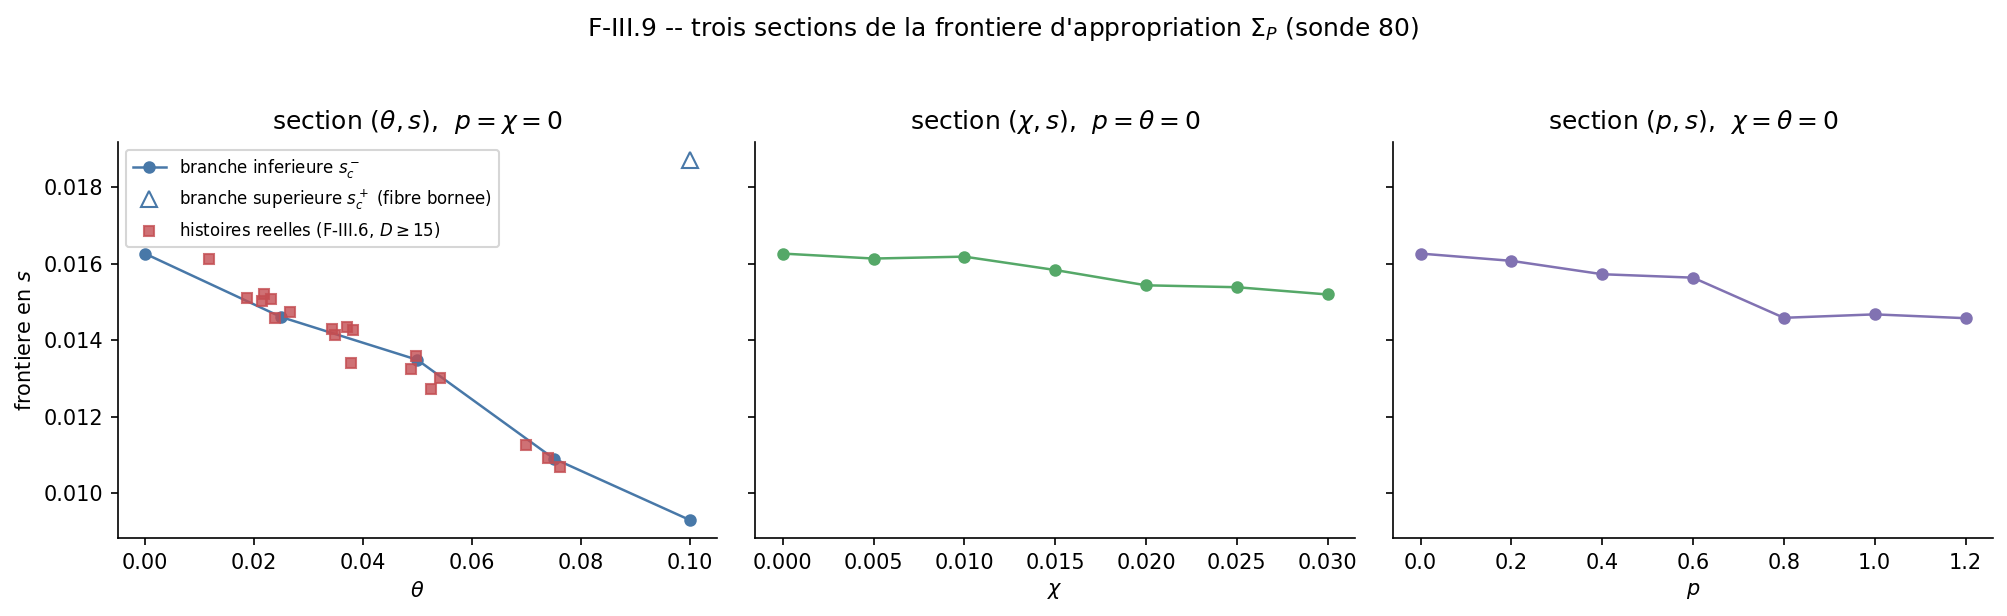
\includegraphics[width=0.96\textwidth]{fig/scientifiques/figure_frontiere_reponse.png}
\caption{Exemple numérique de sections d'une frontière de réponse pour une sonde fixée. La première coupe montre la branche de seuil sur la section alignée ; les deux autres montrent sa variation lorsque des variables lentes résiduelles sont conservées. La construction et les contrôles numériques sont donnés à l'Annexe~I.}
\label{fig:t3-frontiere-reponse}
\end{figure}

\section{Régions de réponse}
\label{t3-regions-reponse}

Considérons une famille de sondes paramétrées par $u\in\Omega$. À chaque valeur de $u$ correspond une histoire de sonde \(\mathcal H_u\). On fixe une réalisation $X$ et une lecture $\rho$. Pour chaque $u$, la sonde produit une réponse \(\mathcal R_X^\rho(\mathcal H_u)\).

Supposons d'abord que la lecture distingue un ensemble discret de réponses. Il peut s'agir, par exemple, du bassin atteint après relaxation, d'un type d'événement, ou d'une catégorie d'issue retenue par le protocole.

Pour une réponse $A$, on définit
\[
S_A(X)
=
\left\{
u\in\Omega
\; ; \;
\mathcal R_X^\rho(\mathcal H_u)=A
\right\}.
\]

L'ensemble $S_A(X)$ rassemble donc les sondes de la famille qui produisent la réponse $A$ depuis la réalisation $X$.

Il s'agit d'une région de l'espace des sondes. Deux valeurs proches de $u$ peuvent appartenir à la même région. Elles produisent alors la même réponse. Elles peuvent aussi appartenir à deux régions différentes. Une faible variation de la sonde suffit alors à changer d'issue. La forme de ces régions donne une première description de l'organisation du profil de réponse dans la famille étudiée.

\section{Comparer deux frontières}
\label{t3-comparer-deux-frontieres}

Soient deux réalisations $X_1$ et $X_2$ interrogées par la même famille
de sondes
\[
u\in\Omega
\longmapsto
\mathcal H_u,
\]
avec la même lecture $\rho$.

Pour une réponse $A$, elles définissent deux régions
\[
S_A(X_1)
\qquad\text{et}\qquad
S_A(X_2),
\]
et leurs frontières
\[
\partial_\Omega S_A(X_1)
\qquad\text{et}\qquad
\partial_\Omega S_A(X_2).
\]

La comparaison la plus simple consiste à demander si ces régions coïncident.

Si
\[
S_A(X_1)=S_A(X_2),
\]
la réponse $A$ est obtenue par les mêmes sondes dans les deux réalisations.

Si
\[
S_A(X_1)\neq S_A(X_2),
\]
il existe au contraire au moins une sonde qui conduit à $A$ depuis une réalisation et pas depuis l'autre. Cette différence peut apparaître sans que la réponse $A$ ait disparu.
Par exemple, les deux régions peuvent rester non vides,
\[
S_A(X_1)\neq\varnothing,
\qquad
S_A(X_2)\neq\varnothing,
\]
tout en occupant des parties différentes de $\Omega$.

La réponse reste alors accessible dans les deux cas, mais les conditions qui permettent de l'obtenir ont changé.

On peut examiner plus précisément leurs frontières.

Si
\[
\partial_\Omega S_A(X_1)
\neq
\partial_\Omega S_A(X_2),
\]
les bascules entre $A$ et les réponses voisines ne se produisent plus aux mêmes endroits dans l'espace des sondes.

Cette comparaison ne suppose pas encore que la frontière soit lisse, ni même qu'elle puisse être décrite par une fonction. Elle demande seulement que les régions de réponse soient définies dans le même espace $\Omega$ et avec la même lecture.

La différence entre deux frontières constitue ainsi une description plus précise qu'une simple différence d'accessibilité. Elle indique non seulement qu'une réponse peut être obtenue, mais que les conditions de son obtention ont été réorganisées.

\section{Ce qu'une frontière permet de dire}
\label{t3-ce-que-frontiere-permet-dire}

Une frontière de réponse n'est pas une frontière interne du système. Elle est construite à partir d'une famille de sondes et d'une lecture déclarées.

Une autre famille de sondes peut révéler une organisation différente.

Une lecture plus grossière peut également réunir des réponses que la
lecture précédente distinguait.

La frontière
\[
\partial_\Omega S_A(X)
\]
doit donc toujours être comprise relativement à
\[
(X,\Omega,\rho).
\]

Sa modification montre qu'une différence fonctionnelle est devenue visible dans la famille étudiée.

Elle ne permet pas, à elle seule, d'identifier la transformation interne qui l'a produite. Cette prudence est importante, deux mécanismes internes différents peuvent déplacer une frontière de la même manière.

Inversement, une transformation interne peut rester invisible si la
famille de sondes ne rencontre pas la région où ses effets apparaissent.

Les frontières ne donnent donc pas accès directement au terrain. Elles en fournissent une image fonctionnelle, construite à partir des réponses du système.

\section{Trois niveaux de changement}
\label{t3-trois-niveaux-changement}

Une histoire peut modifier une région de réponse de plusieurs manières. Toutes ces modifications ne portent pas sur le même aspect de sa géométrie.

On peut distinguer trois niveaux.

\subsection{Déplacement}

Le cas le plus simple est celui d'une frontière qui change de position sans que son organisation générale soit modifiée.

Considérons une famille de sondes décrite par un paramètre scalaire
\[
u\in\Omega\subset\mathbb R.
\]

Supposons que la réponse $A$ soit obtenue pour
\[
u<u^\ast.
\]

La frontière est alors située en
\[
u=u^\ast.
\]

Après une histoire $\mathcal H_0$, on peut obtenir un nouveau seuil
\[
u=u^\ast_{\mathcal H_0}.
\]

Si
\[
u^\ast_{\mathcal H_0}\neq u^\ast,
\]
la frontière s'est déplacée.

La même bascule existe encore, mais elle ne se produit plus pour la même sonde. Ce déplacement suffit à montrer que l'histoire a modifié les conditions d'obtention de la réponse.

\subsection{Déformation}

Lorsque l'espace des sondes possède plusieurs dimensions, une frontière ne se réduit généralement plus à un seuil.

Pour
\[
u\in\Omega\subset\mathbb R^m,
\qquad m\geq 2,
\]
dans les cas réguliers, la frontière peut former une courbe ou une surface ; sans hypothèse supplémentaire de régularité, elle peut être un ensemble plus complexe. Deux réalisations peuvent alors présenter des frontières différentes sans que cette différence se résume à un déplacement uniforme. Certaines parties peuvent avancer, d'autres reculer.

La forme de la région de réponse change. Nous parlerons alors de déformation. Cette notion reste descriptive, elle indique que la modification dépend de la direction dans laquelle la famille de sondes est explorée.

\subsection{Changement d'organisation}

Une transformation plus profonde apparaît lorsque la différence ne porte plus seulement sur la position ou la forme d'une frontière.

Le nombre de régions non vides peut changer. Une région peut apparaître ou disparaître. Deux régions auparavant non voisines peuvent devenir voisines, ou leurs adhérences entrer en contact.

Une même réponse peut également occuper plusieurs composantes disjointes de l'espace des sondes.

Dans ces situations, l'organisation des régions de réponse elle-même a changé. Nous parlerons de changement d'organisation.

Cette distinction ne constitue pas encore une classification
mathématique complète.

Elle sépare seulement trois questions :

\begin{itemize}
\tightlist
\item
  la bascule a-t-elle changé de position ?
\item
  sa forme a-t-elle changé ?
\item
  l'organisation des régions a-t-elle changé ?
\end{itemize}

Ces trois niveaux peuvent se combiner.

Une histoire peut déplacer une frontière, la déformer et modifier en même temps l'organisation des régions qu'elle sépare.

\section{Changer de frontière sans changer de réponse}
\label{t3-changer-frontiere-sans-changer-reponse}

Une modification des frontières n'implique pas nécessairement
l'apparition d'une nouvelle réponse.

Supposons que deux réalisations possèdent le même ensemble de réponses
accessibles :
\[
\operatorname{Acc}_{\mathfrak B,\rho}(X_1)
=
\operatorname{Acc}_{\mathfrak B,\rho}(X_2).
\]

Cette égalité ne dit pas quelles sondes produisent chacune de ces
réponses.

On peut donc avoir, pour une réponse $A$,
\[
S_A(X_1)\neq S_A(X_2),
\]
alors même que
\[
S_A(X_1)\neq\varnothing,
\qquad
S_A(X_2)\neq\varnothing.
\]

Aucune possibilité n'a nécessairement été créée ou supprimée. C'est leur répartition dans l'espace des sondes qui a changé. Cette situation est importante pour l'étude de l'histoire.

Une transformation persistante peut devenir visible non parce que le
système possède de nouvelles réponses, mais parce que les conditions
nécessaires pour atteindre les réponses déjà présentes ont été
modifiées.

\section{Même organisation, géométrie différente}
\label{t3-meme-organisation-geometrie-differente}

Deux réalisations peuvent produire des régions de réponse de formes différentes sans que leur organisation générale soit modifiée.

Considérons deux réalisations $X_1$ et $X_2$, interrogées par la même famille de sondes et avec la même lecture.

Pour chaque réponse $A$, elles définissent les régions
\[
S_A(X_1)
\qquad\text{et}\qquad
S_A(X_2).
\]

Supposons que les mêmes réponses soient présentes dans les deux cas.

Les régions peuvent changer de taille ou de forme. Leurs frontières peuvent également se déplacer. Cela ne suffit pas à montrer que leur organisation a changé.

Par exemple, une région associée à $A$ peut rester voisine des mêmes régions, même si les frontières qui les séparent ont été déformées. De même, une région peut s'étendre ou se contracter sans apparaître, disparaître ou se séparer en plusieurs parties.

Dans ces situations, la géométrie a changé, mais certaines relations
entre les régions ont été conservées.

Nous dirons alors que les deux découpages possèdent la même organisation au niveau considéré.

Cette expression reste volontairement relative.

Le niveau considéré doit préciser quelles propriétés sont retenues : présence des régions, nombre de composantes, voisinages entre réponses, ou autre propriété déclarée par le protocole.

Deux découpages peuvent donc être considérés comme équivalents à un niveau et différents à un niveau plus fin.

\section{Le graphe des voisinages}
\label{t3-graphe-voisinages}

Une première description de l'organisation des régions consiste à retenir seulement leurs voisinages.

On associe à une réalisation $X$ un graphe
\[
\mathcal G_{\Omega,\rho}(X).
\]

Ses sommets correspondent aux réponses dont la région est non vide :
\[
S_A(X)\neq\varnothing.
\]

Deux sommets \(A\) et \(B\) sont reliés lorsque les régions correspondantes sont voisines au sens du découpage : elles partagent localement une séparation effective. Un simple contact isolé de leurs adhérences n'est pas compté comme une arête.

Le graphe ne conserve ni la position des frontières, ni leur forme. Il retient seulement quelles réponses peuvent se rencontrer dans le
découpage considéré.

Une déformation peut donc modifier les ensembles
\[
S_A(X)
\]
sans modifier
\[
\mathcal G_{\Omega,\rho}(X).
\]

Dans ce cas, la géométrie a changé, mais les voisinages entre réponses ont été conservés.

À l'inverse, si
\[
\mathcal G_{\Omega,\rho}(X_1)
\not\simeq
\mathcal G_{\Omega,\rho}(X_2),
\]
alors l'organisation des voisinages a changé.

Une telle différence ne peut plus être décrite par le seul déplacement des frontières.

\section{Reconnaître un changement d'organisation}
\label{t3-reconnaitre-changement-organisation}

Le graphe des voisinages fournit un premier moyen de détecter certains changements d'organisation.

D'autres peuvent être observés directement sur les régions.

Pour une réponse $A$, plusieurs situations peuvent notamment apparaître :

\begin{itemize}
\tightlist
\item
  $S_A(X)$ devient vide ou cesse de l'être ;
\item
  le nombre de ses composantes change ;
\item
  ses voisinages avec les autres régions changent.
\end{itemize}

Ces modifications ne décrivent pas simplement une frontière qui se déplace. Elles indiquent qu'une propriété du découpage retenue par le protocole n'est plus conservée.

On parlera alors de changement d'organisation au niveau considéré. Cette notion ne cherche pas encore à expliquer le mécanisme responsable du changement.

Elle permet seulement de distinguer deux situations :

\[
\text{la géométrie change mais l'organisation retenue demeure},
\]

ou

\[
\text{une propriété retenue de l'organisation change elle aussi}.
\]

La seconde situation marque un changement qualitatif dans la structure des réponses observées.

\section{Lorsque la frontière cesse d'être simple}
\label{t3-frontiere-cesse-etre-simple}

Jusqu'ici, aucune régularité particulière n'a été imposée aux frontières
de réponse.

Dans les situations les plus simples, une frontière sépare localement
deux régions et varie de manière régulière dans l'espace des sondes.

Cette situation n'est pas générale. Une frontière peut se replier. Plusieurs portions de frontière peuvent se rencontrer. Une même réponse peut apparaître de part et d'autre d'une autre région.

Ces configurations demandent davantage d'information que la seule
position de la frontière. Elles demandent aussi davantage que le graphe des voisinages.

Deux découpages peuvent en effet posséder les mêmes régions et les mêmes relations de voisinage, tout en différant par la manière dont leurs frontières sont organisées localement.

Nous distinguerons deux situations utiles pour la suite : le pli et la couture. Ces termes décrivent des propriétés locales du découpage dans l'espace des sondes. Ils ne désignent pas, à eux seuls, les mécanismes internes qui les ont produites.

\section{Pli d'une frontière de réponse}
\label{t3-pli-frontiere-reponse}

Considérons d'abord une coupe unidimensionnelle de l'espace des sondes.

Dans le cas le plus simple, une réponse change une seule fois lorsque le
paramètre $u$ varie.

On peut alors rencontrer une succession du type
\[
A \;|\; B.
\]

Une configuration différente apparaît lorsqu'une même réponse est
rencontrée de nouveau après avoir traversé une autre région :
\[
A \;|\; B \;|\; A.
\]

La région associée à $B$ est alors encadrée, dans cette coupe, par deux bascules. Cette observation peut être produite par une géométrie de frontière qui se replie par rapport à la direction explorée.

Nous parlerons de pli lorsqu'une telle structure résulte localement de la géométrie de la frontière dans l'espace des sondes. Le pli ne crée pas nécessairement une nouvelle réponse. Il peut modifier seulement la manière dont des réponses déjà accessibles sont distribuées dans $\Omega$. Il dépend également de la famille de sondes choisie.

Une coupe peut révéler plusieurs bascules là où une autre direction d'exploration en révèle une seule. Le pli doit donc être interprété comme une propriété géométrique relative au protocole de sondage.

La succession
\[
A \;|\; B \;|\; A
\]
constitue ainsi un indice de pli dans la coupe considérée. Elle ne suffit pas, à elle seule, à caractériser la géométrie complète de la frontière.

\section{Pli et histoire}
\label{t3-pli-et-histoire}

Un pli devient intéressant pour l'étude de l'histoire lorsque sa présence dépend de la réalisation interrogée.

Soient deux réalisations $X_1$ et $X_2$ obtenues avant et après le
contraste historique défini précédemment. Une même famille de sondes peut produire, pour $X_1$, une séparation simple entre deux réponses, puis révéler pour $X_2$ une région encadrée par deux bascules.

L'histoire n'a alors pas nécessairement modifié l'ensemble des réponses accessibles. Elle a modifié leur organisation dans l'espace des sondes. Inversement, un pli déjà présent peut être déplacé, déformé ou disparaître.

L'objet de la comparaison n'est donc pas le pli pris isolément. C'est la différence entre les géométries de réponse portées par les deux réalisations.

\section{Lorsque les régions se rencontrent}
\label{t3-lorsque-regions-se-rencontrent}

Le graphe des voisinages indique quelles régions de réponse sont en relation. Il ne précise pas comment cette relation se produit.

Deux régions peuvent être séparées par une portion de frontière commune. Dans les cas réguliers, elles peuvent aussi ne se rencontrer qu'en un point, ou le long d'un ensemble de dimension plus faible. Ces situations ne doivent pas être confondues.

Considérons deux réponses $A$ et $B$ et leurs régions
\[
S_A(X)
\qquad\text{et}\qquad
S_B(X).
\]

Le simple fait que leurs adhérences se rencontrent,
\[
\overline{S_A(X)}
\cap
\overline{S_B(X)}
\neq
\varnothing,
\]
établit un contact.

Il ne suffit pas encore à décrire la nature de ce contact.

Dans une situation régulière, les deux régions peuvent partager localement une même frontière. De part et d'autre de cette frontière, la réponse passe alors de $A$ à $B$. Mais une rencontre peut aussi être plus localisée. Plusieurs régions peuvent atteindre le même point sans partager autour de ce point une même portion de séparation. La distinction entre contact et voisinage dépend donc de la géométrie retenue par le protocole.

Pour la suite, nous réserverons le terme de voisinage aux rencontres qui correspondent à une séparation effective entre deux régions dans l'espace des sondes. Un contact isolé ne sera pas, à lui seul, considéré comme un voisinage.

\section{Rencontre de plusieurs réponses}
\label{t3-rencontre-plusieurs-reponses}

Une frontière régulière sépare localement deux régions de réponse. D'autres configurations peuvent faire intervenir davantage de régions.

Il peut exister un point
\[
u^\ast\in\Omega
\]
au voisinage duquel plusieurs réponses sont présentes.

Pour trois réponses $A$, $B$ et $C$, on peut par exemple avoir
\[
u^\ast
\in
\overline{S_A(X)}
\cap
\overline{S_B(X)}
\cap
\overline{S_C(X)}.
\]

Cette condition indique que les trois régions atteignent le même point. Elle ne précise pas encore comment elles s'y organisent. Le point peut correspondre à la rencontre de plusieurs frontières.
Il peut aussi apparaître parce que l'une des régions se termine, se sépare ou devient trop mince pour persister au-delà de ce voisinage. La seule liste des réponses présentes ne suffit donc plus. Il faut examiner la manière dont leurs régions se raccordent autour de $u^\ast$.

\section{Couture de régions de réponse}
\label{t3-couture-regions-reponse}

Nous appellerons couture une configuration locale dans laquelle le raccordement entre régions de réponse ne peut plus être décrit par une unique séparation régulière entre deux régions.

Une couture peut notamment apparaître lorsque plusieurs portions de frontière se rejoignent ou lorsqu'une région se termine au contact d'autres régions.

Le point essentiel n'est pas le nombre de réponses présentes. C'est la manière dont leurs frontières se raccordent localement. Comme pour le pli, la couture est définie relativement à la famille de sondes et à la lecture retenues.

Elle ne désigne pas directement une singularité interne du système. Elle décrit une singularité de l'organisation des réponses observées dans l'espace des sondes.
Une formalisation plus forte, fondée sur la signature combinatoire des exécutions hybrides, est donnée à l'Annexe~\ref{annexe-geometrie-frontiere-commutation}. La Proposition~\ref{prop:J-pli-couture} y distingue les déformations qui restent dans une même cellule d'exécution des raccords qui rencontrent un changement de signature. 

\part{Ce que la géométrie permet de distinguer}

\chapter{Lire une géométrie de réponse}
\begin{figure}[htbp]
\centering
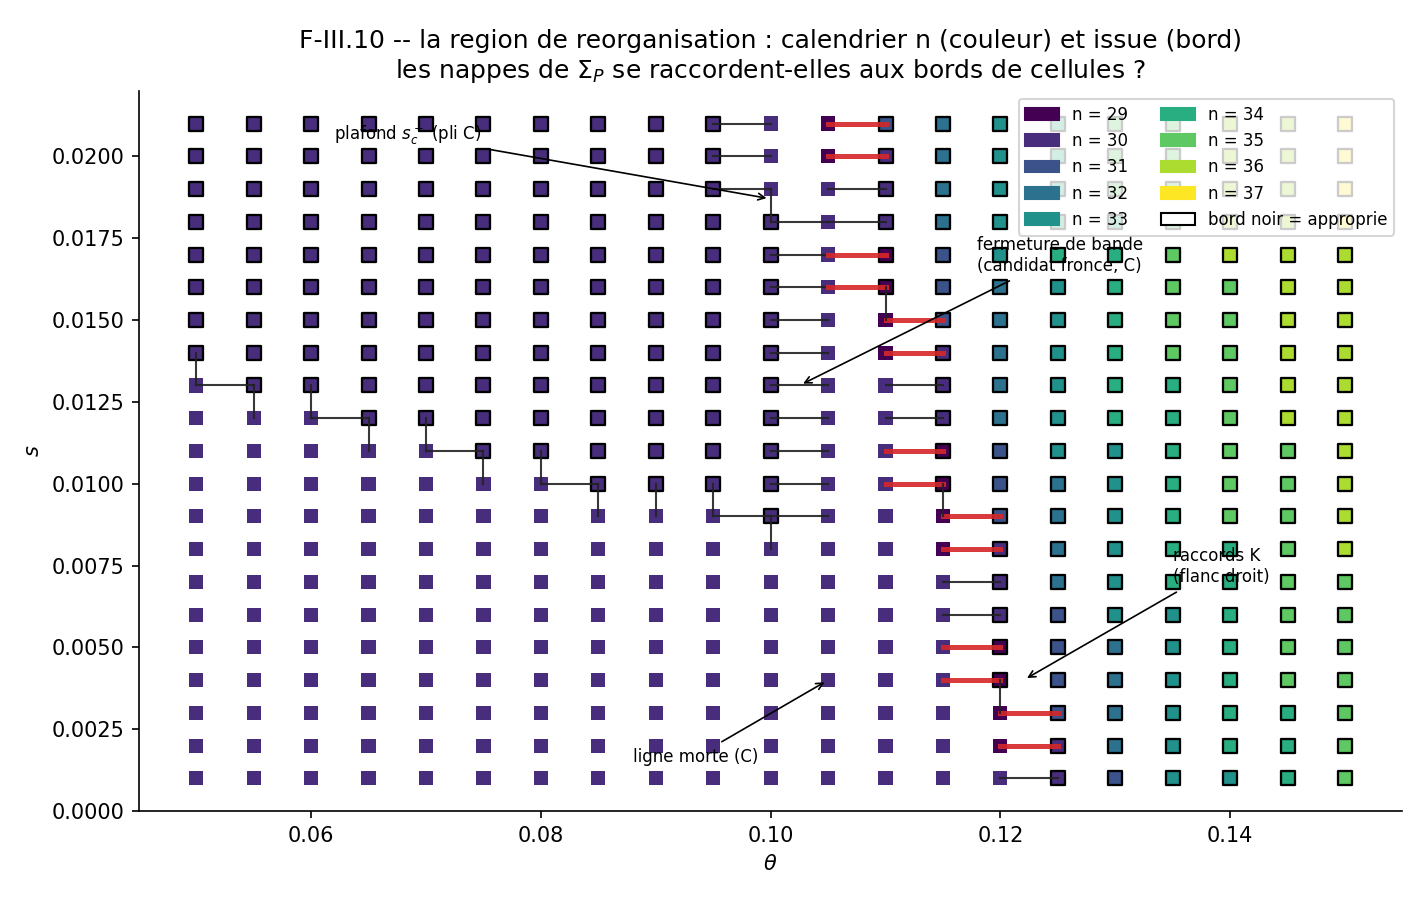
\includegraphics[width=0.90\textwidth]{fig/scientifiques/figure_raccord_frontiere.png}
\caption{Carte numérique d'un raccord de régions de réponse dans un plan de sondes. La couleur code le calendrier événementiel et le bord la classe d'issue ; les changements de calendrier et les changements d'issue ne coïncident donc pas partout. Ce cas sert de contrôle à la distinction entre recomposition hybride et déformation continue développée à l'Annexe~J.}
\label{fig:t3-raccord-frontiere}
\end{figure}

\section{Ce que les frontières permettent d'inférer}\label{t3-inference-frontieres}

Les régions de réponse, leurs frontières et leurs singularités
constituent des objets d'observation. Ils permettent de comparer des réalisations, de suivre les effets d'une histoire et de décrire l'organisation des réponses dans une famille de sondes. Ils ne décrivent cependant pas directement l'organisation interne du système. Une même géométrie de réponse peut être produite par plusieurs mécanismes internes.

Inversement, une modification interne peut rester invisible si elle ne change aucune des réponses observées dans le protocole retenu. L'interprétation d'une géométrie de réponse demande donc de distinguer avec soin ce qui est observé de ce qui est inféré.

\section{Une même géométrie n'identifie pas une histoire}
\label{t3-geometrie-n-identifie-pas-histoire}

Considérons deux histoires
\[
\mathcal H_1
\qquad\text{et}\qquad
\mathcal H_2.
\]

Appliquées à une même réalisation initiale, elles conduisent à deux
réalisations finales
\[
X_1
=
\Phi_{\mathcal H_1}(X_0),
\qquad
X_2
=
\Phi_{\mathcal H_2}(X_0).
\]

Supposons que, pour toute réponse \(A\),

\[
S_A(X_1)=S_A(X_2)
\]

dans la famille de sondes considérée. Les deux réalisations donnent alors la même réponse pour toute sonde de cette famille. Elles sont équivalentes en réponse pour le protocole déclaré, et leur géométrie de réponse est identique.

Cela ne permet pas de conclure que

\[
\mathcal H_1=\mathcal H_2.
\]

Deux histoires distinctes peuvent conduire à des réalisations indiscernables pour le protocole déclaré.

La géométrie de réponse caractérise donc une classe d'observations. Elle ne constitue pas une signature unique de l'histoire.

\section{Une même réalisation peut produire plusieurs géométries}
\label{t3-meme-histoire-plusieurs-geometries}

La géométrie observée dépend également du protocole. Une même réalisation peut être interrogée par deux familles de sondes différentes. Les régions obtenues dans les deux expériences ne sont alors pas nécessairement comparables.

Certaines frontières peuvent rester invisibles dans une première exploration. D'autres peuvent apparaître lorsque la famille de sondes est enrichie ou explore d'autres directions. Une géométrie de réponse n'est donc jamais absolue. Elle est toujours relative à la famille de sondes et à la lecture déclarées.

\paragraph*{Géométrie de réponse}

Soit un protocole d'observation déclaré \((\mathfrak B,\rho)\), dans
lequel la famille de sondes est paramétrée par

\[
u\in\Omega\subset\mathbb R^m.
\]

La \emph{géométrie de réponse} d'une réalisation \(X\) est
l'organisation des régions

\[
S_A(X)\subset\Omega
\]

et de leurs frontières relativement à ce protocole déclaré.
    

\paragraph*{Principe de prudence observationnelle}


La géométrie de réponse est un objet d'observation. Elle ne doit pas être confondue avec l'organisation interne du système.

Deux propriétés fondamentales en découlent.

\begin{enumerate}
\item \textbf{Sous-détermination.}

Une même géométrie de réponse peut être compatible avec plusieurs organisations internes. La géométrie de réponse ne détermine donc pas, à elle seule, le monde intérieur.

\item \textbf{Non-absoluité.}

Une même réalisation peut conduire à des géométries de réponse différentes lorsque le protocole d'observation $(\mathfrak B,\rho)$ est modifié. La géométrie de réponse n'est donc jamais une propriété absolue du système. Elle est toujours relative au protocole déclaré.
\end{enumerate}

Toute interprétation d'une géométrie de réponse doit donc distinguer avec soin ce qui est effectivement observé de ce qui est inféré sur l'organisation interne du système.

La plasticité fournit une instance exacte de cette sous-détermination. Sous réalisabilité causale et markovienne, une présentation à loi plastique et une présentation à loi figée munie d'une coordonnée d'état supplémentaire peuvent produire les mêmes exécutions et les mêmes réponses. Leur équivalence est établie à l'Annexe~\ref{annexe-equivalence-presentation-plasticite} (Théorème~\ref{thm:K-equivalence-plasticite}).

\section{La géométrie de réponse comme invariant relatif}
\label{t3-geometrie-invariant-relatif}

Pour un protocole déclaré, deux réalisations équivalentes en réponse produisent la même géométrie de réponse. Celle-ci peut donc être comprise comme un invariant de la classe d'équivalence en réponse, relativement au protocole considéré.

Cet invariant ne décrit pas le détail des transformations subies par le système. Plusieurs histoires distinctes peuvent conduire à des réalisations portant la même géométrie de réponse.

La géométrie de réponse peut ainsi être comprise comme un invariant relatif au protocole déclaré. Le qualificatif « relatif » est essentiel. Il rappelle que cet invariant dépend de la famille de sondes et de la lecture choisies.

Modifier le protocole peut faire apparaître de nouvelles distinctions ou, au contraire, en faire disparaître certaines.

L'invariance ne porte donc jamais sur le système seul. Elle porte sur ce qui reste inchangé dans l'observation du système.

\subsection*{Conséquence}

L'histoire ne se réduit donc pas à la suite des épisodes qui la composent. Elle peut également être étudiée par les invariants qu'elle préserve ou par ceux qu'elle modifie.

Deux histoires peuvent différer sans que cette différence soit visible dans la géométrie de réponse. Inversement, une modification de la géométrie de réponse atteste qu'une propriété observable du système a été transformée.

\section{Les histoires et les changements de géométrie}
\label{t3-histoires-changements-geometries}

Jusqu'à présent, une histoire a été étudiée à travers la réalisation qu'elle produit. La géométrie de réponse permet d'adopter un point de vue différent.

Au lieu de comparer directement deux réalisations, on peut comparer les géométries de réponse qu'elles induisent dans un même protocole d'observation.

Pour une réalisation donnée, une histoire permet de comparer la géométrie de réponse avant et après la transformation qu'elle produit. L'objet de la comparaison n'est plus seulement l'état atteint, mais la manière dont l'organisation des réponses a été modifiée.

Soit une histoire \(\mathcal H\) et une réalisation initiale \(X\).
Dans un même protocole d'observation, on compare la géométrie de réponse de \(X\) à celle de

\[
\Phi_{\mathcal H}(X).
\]

La part de l'effet de l'histoire rendue visible par cette géométrie est contenue dans cette comparaison.

Certaines histoires ne modifient pas la géométrie de réponse. D'autres déplacent des frontières sans modifier leur organisation. D'autres encore changent la structure même des régions de réponse.

La géométrie de réponse fournit ainsi une première classification des
effets observables d'une histoire.

\section{Transformations observables et propriétés préservées}
\label{t3-transformations-observables}

Une histoire ne modifie pas nécessairement tous les aspects d'une géométrie de réponse. Certaines propriétés peuvent être préservées tandis que d'autres sont transformées.

L'étude d'une histoire ne consiste donc pas seulement à décrire les changements qu'elle produit. Elle consiste également à identifier les propriétés qui demeurent inchangées. Ces propriétés préservées dépendent du niveau d'observation retenu.

Ainsi, une histoire peut déplacer une frontière tout en conservant l'organisation des régions de réponse. Elle peut également modifier cette organisation sans changer l'ensemble des réponses accessibles.

L'analyse d'une histoire revient donc à comparer simultanément les propriétés conservées et les propriétés transformées de la géométrie de réponse.

On peut distinguer plusieurs niveaux de transformation.

\begin{itemize}
\tightlist
\item
une transformation peut laisser inchangée la géométrie de réponse ;

\item
elle peut modifier la position des frontières tout en conservant leur
organisation ;

\item
elle peut modifier l'organisation des régions de réponse ;

\item
elle peut enfin faire apparaître ou disparaître des réponses
accessibles.
\end{itemize}

Ces niveaux ne constituent pas une hiérarchie absolue. Ils décrivent simplement des modifications de plus en plus structurantes dans la géométrie de réponse relative au protocole considéré.

\section{Une notion d'équivalence}
\label{t3-notion-equivalence}

La géométrie de réponse ne demande pas d'introduire une nouvelle notion d'équivalence. On reprend l'équivalence en réponse définie à la section~\ref{t3-equivalence-declaree} :

\[
X\sim_{\mathfrak B,\rho}Y
\quad\Longleftrightarrow\quad
\forall\mathcal H\in\mathfrak B,
\qquad
\mathcal R_X^\rho(\mathcal H)
=
\mathcal R_Y^\rho(\mathcal H).
\]

Dans le cas d'une famille paramétrée
\[
\mathfrak B_\Omega
=
\{\mathcal H_u\,;\,u\in\Omega\}
\]
et d'une lecture discrète, cette égalité revient à demander

\[
S_A(X)=S_A(Y)
\]

pour toute réponse \(A\).

Deux réalisations distinctes peuvent donc appartenir à la même classe d'équivalence en réponse. La géométrie observée ne les identifie pas comme objets internes ; elle indique seulement qu'aucune sonde du protocole déclaré ne les sépare.

Lorsque les histoires admissibles sont en outre munies d'une mesure de complexité \(c\), cette question peut être graduée : non plus seulement \emph{les deux réalisations sont-elles séparables ?}, mais \emph{à quelle profondeur une histoire séparatrice apparaît-elle ?}

La profondeur de séparabilité
\[
\ell_{c,\mathfrak B,\rho}(X,Y)
\]
et l'ultramétrique qu'elle induit sur le quotient d'observation sont construites à l'Annexe~\ref{annexe-ultrametrique-separabilite}. Cette géométrie reste relative à la classe d'histoires, à la lecture et à la complexité déclarées ; elle ne définit pas une distance physique entre états.

\begin{figure}[htbp]
\centering
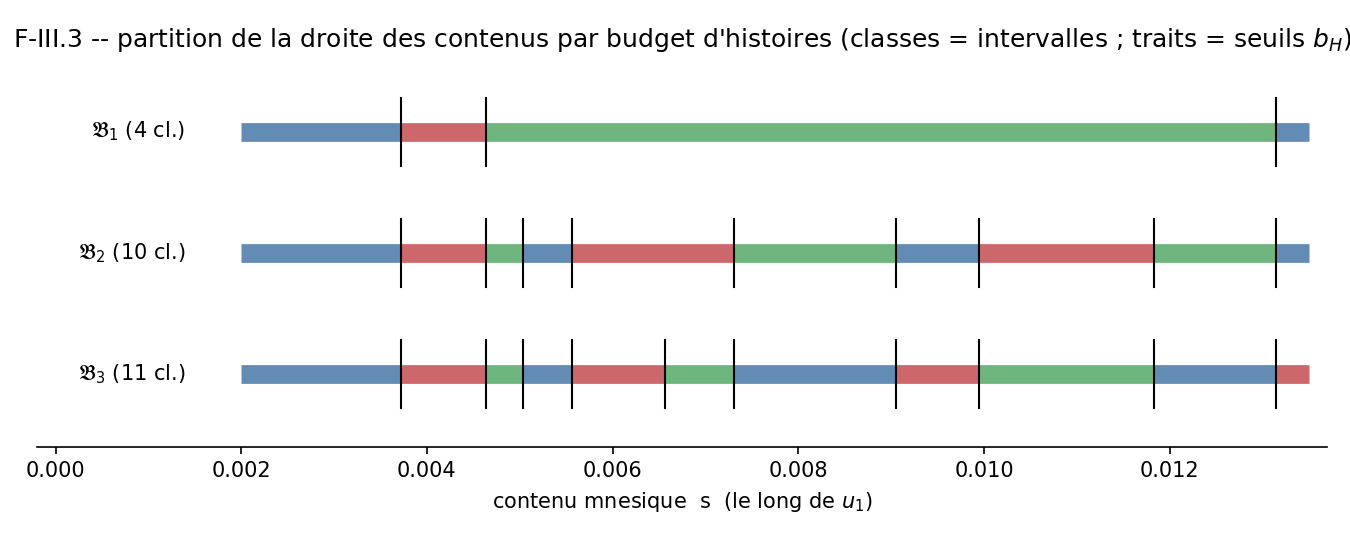
\includegraphics[width=0.88\textwidth]{fig/scientifiques/figure_separabilite_budgets.png}
\caption{Filtration d'un même espace de contenus par trois budgets d'histoires. Les traits verticaux marquent les seuils où les classes d'indiscernabilité changent. L'emboîtement obtenu est la manifestation numérique de la hiérarchie de séparabilité formalisée à l'Annexe~\ref{annexe-ultrametrique-separabilite}.}
\label{fig:t3-separabilite-budgets}
\end{figure}

\section{Ce que l'observation laisse ouvert}

Une équivalence en réponse ne ferme pas la description d'une réalisation. Elle indique seulement qu'au regard du protocole déclaré, aucune distinction supplémentaire n'a été obtenue.

Deux réalisations équivalentes peuvent ainsi demeurer différentes sans que cette différence soit accessible aux sondes considérées. Enrichir la famille de sondes ou modifier la lecture peut alors faire apparaître une séparation jusque-là invisible. Mais rien ne garantit qu'une telle extension existe, ni qu'elle soit accessible dans la classe d'expériences considérée.

La géométrie de réponse doit donc être comprise simultanément par ce qu'elle distingue et par ce qu'elle laisse indéterminé. Ses frontières séparent des réponses observables ; elles ne dessinent pas les frontières du monde intérieur.

Cette limite n'est pas une insuffisance du dispositif. Elle appartient à sa définition. Toute géométrie de réponse est relative à une manière d'interroger le système, et toute conclusion tirée de cette géométrie demeure relative au protocole qui la produit.

Le chemin parcouru dans ce tome peut alors être lu dans l'autre sens. Une histoire transforme une réalisation ; cette transformation peut modifier ce qui lui devient accessible ; les sondes rendent certaines de ces différences observables ; leurs réponses organisent une géométrie ; et cette géométrie détermine enfin ce que, dans le protocole choisi, il est possible de distinguer.

\medskip

\noindent\emph{Un intérieur ne se donne pas tout entier dans ses
réponses. Il se distingue d'un autre lorsque leurs réponses à une même
sonde cessent de coïncider.}